\documentclass[conference]{IEEEtran}
\usepackage{standalone}
\usepackage{times}
\usepackage{float}

%% Additional packages
\usepackage{times}
\usepackage{amsmath}
\usepackage{amsthm}
\usepackage{amssymb}
\usepackage{amsfonts}
\usepackage{mathtools}
%\usepackage{calc}
\usepackage{subfigure}
\usepackage{graphicx}
\usepackage{color}
\usepackage{url}
%\usepackage{lineno}
%\usepackage{ulem} % for underlining and strike through
%\normalem % reset emph to normal
%\usepackage{setspace} % for line spacing - e.g. 1.5, 2
\usepackage[usenames,x11names]{xcolor}
%\usepackage{xspace} % for inserting a space in TeX commands if needed
%\usepackage{caption}
\usepackage[bookmarks=true]{hyperref}
%\renewcommand{\thesubfigure}{\relax} % no subfig counters
%\let\chapter\section % algorithm2e natbib compatibility
%\usepackage{accents}
%\usepackage[titletoc,toc,title]{appendix}
%\usepackage{longtable}
%\usepackage{setspace}
\usepackage{multicol}

%% Packages
%\usepackage[margin=1in]{geometry}
%\usepackage[abs]{overpic}
\usepackage[linesnumbered,vlined,ruled]{algorithm2e}
%\usepackage{multirow} % for cell tables spanning multiple rows
\usepackage{tikz,pgf}%,tikz-3dplot}
\usetikzlibrary{arrows,automata,shapes,calc,backgrounds,spy,positioning}
%\usetikzlibrary{external}
%\tikzexternalize
%\usepackage[numbers]{natbib}
%\usepackage[sort,round]{natbib}
%\usepackage{lipsum}
\usepackage{epstopdf}

\theoremstyle{plain}
\newtheorem{theorem}{Theorem}
\newtheorem{cor}{Corollary}
\newtheorem{prop}{Proposition}
\newtheorem{lemma}{Lemma}

\theoremstyle{definition}
%\newtheorem{definition}{Definition}
\newtheorem{remark}{Remark}
\newtheorem{cond}{Condition}

\newtheorem{example}{Example}
\newtheorem{problem}{Problem}
%\newtheorem{assumption}{Assumption}


%%% figure path
\graphicspath{{figures/}}

%% Remove footnote mark
%\renewcommand{\footnotemark}{}

%%% Redefine qed symbol
%\renewcommand{\qedsymbol}{$\blacksquare$}

%% Projection symbol
%\newcommand{\project}[1]{\! \upharpoonright_{#1}}


%% Theorems 
%\newtheorem{theorem}{Theorem}[section]
%\newtheorem{proposition}[theorem]{Proposition}
%\newtheorem{corollary}[theorem]{Corollary}
\newtheorem{definition}[theorem]{Definition}
%\newtheorem{lemma}[theorem]{Lemma}
%\newtheorem{remark}[theorem]{Remark}
%\newtheorem{remarks}[theorem]{Remarks}
%\newtheorem{example}[theorem]{Example}
%\newtheorem{algo}[theorem]{Algorithm}
%\newtheorem{problem}[theorem]{Problem}
%\newtheorem{Procedure}[theorem]{Procedure}
%\newcommand{\exampler}[2]{\medskip \hskip -\parindent {\bf Example #1 Revisited.~}{\it #2}\medskip}

%% Percent
%\newcommand\oprocendsymbol{\hbox{$\square$}}
%\newcommand\oprocend{\relax\ifmmode\else\unskip\hfill\fi\oprocendsymbol}
%\def\eqoprocend{\tag*{$\bullet$}}

%% Enumerate environment
%\renewcommand{\labelenumi}{(\roman{enumi})}
%\renewcommand{\labelenumii}{(\alph{enumii})}

%% Breakable comma
%\mathchardef\breakingcomma\mathcode`\,
%{\catcode`,=\active
%  \gdef,{\breakingcomma\discretionary{}{}{}}
%}
%\newcommand{\breqn}[1]{\mathcode`\,=\string"8000 #1}

%% Other Stuff
%\newcommand{\margin}[1]{\marginpar{\tiny\color{blue} #1}}
%%\addtolength{\marginparwidth}{-0.3in}
\newcommand{\todo}[1]{\vskip 0.05in \colorbox{yellow}{$\Box$ \ttfamily\bfseries\small#1}\vskip 0.05in}
%\newcommand{\todo}[1]{}
%\newcommand{\vers}{\operatorname{vers}}

%% Roman, calligraphic, boldface, double barred letters
\newcommand{\RM}[1]{\mathrm{#1}}
\newcommand{\CA}[1]{\mathcal{#1}}
\newcommand{\BF}[1]{\mathbf{#1}}
\newcommand{\IT}[1]{\mathit{#1}}
\newcommand{\BB}[1]{\mathbb{#1}}
\newcommand{\TT}[1]{\mathtt{#1}}
\newcommand{\FK}[1]{\mathfrak{#1}}
\newcommand{\BS}[1]{\boldsymbol{#1}}

%%% Temporal logic symbols
\newcommand{\notltl}{\neg}
\newcommand{\andltl}{\wedge}
\newcommand{\orltl}{\vee}
\newcommand{\Next}{\ensuremath{\bigcirc}}
\newcommand{\Always}{\ensuremath{\ \square\ }}
\newcommand{\Event}{\ensuremath{\ \diamondsuit\ }}
\newcommand{\Until}{\ \CA{U}\ }
\newcommand{\Implies}{\Rightarrow}
\newcommand{\Equiv}{\Leftrightarrow}
%\newcommand{\Not}{\lnot}
\newcommand{\True}{\top}
\newcommand{\False}{\perp}
%\def\prop{\TT{data}}
%\def\popt{\pi}
\newcommand{\AP}{AP}
\newcommand{\pred}{\xi}

\newcommand{\Real}{\BB{R}}

%% Abbreviations
%\def\eg{e.g.\xspace}
%\def\Eg{E.g.\xspace}
%\def\ie{i.e.\xspace}
%\def\Ie{I.e.\xspace}
%\def\etc{etc.\xspace}
%\def\vs{vs.\xspace}
%\def\wrt{w.r.t.\xspace}
%\def\etal{et al.\xspace}

%% Exotic words
\newcommand{\buchi}{B\"uchi\ }

%% Symbols of automata
\newcommand{\PA}{\mathcal{P}}
\newcommand{\BA}{\mathcal{B}}
%\newcommand{\FA}{\mathcal{F}}

\newcommand{\TS}{\mathcal{F}}
\newcommand{\LA}{\mathcal{L}}
\newcommand{\KA}{\mathcal{K}}
\newcommand{\MDP}{\mathcal{M}}
\newcommand{\RA}{\mathcal{R}}
\newcommand{\FSA}{\mathcal{A}}

\newcommand{\TSX}{\BB{V}_\TS}
\newcommand{\TSE}{\BB{E}_\TS}
\newcommand{\TSEE}{\BB{E}}

\newcommand{\DTL}{DTL\xspace}


%% Short macros for arrows
\newcommand{\la}{\leftarrow}
\newcommand{\ra}{\rightarrow}
\newcommand{\ras}[1]{\stackrel{#1}{\rightarrow}}
\newcommand{\asgn}{\la}
\newcommand{\proj}[2]{{#1}{\downharpoonright_{#2}}}

\newcommand{\df}{\xspace\RM{d}}

%% Names of the Algorithms
%\newcommand{\optrun}{\textsc{Optimal-Run}\ }
%\newcommand{\exactmultioptrun}{\textsc{Exact-Multi-Robot-Optimal-Run}\ }
%\newcommand{\constR}{\textsc{Construct-Region-Automaton}\ }
%\newcommand{\constT}{\textsc{Construct-Team-TS}\ }
%\newcommand{\syncT}{\textsc{Sync-Team-TS}\ }
%\newcommand{\boundOpt}{\textsc{Bound-Optimality}\ }

% Custom operators
%\DeclareMathOperator*{\argmin}{arg\,min}
\newcommand{\norm}[1]{\left\| {#1} \right\|}
\newcommand{\norminf}[1]{\left\| {#1} \right\|_{\infty}}
\newcommand{\normeucl}[1]{\left\| {#1} \right\|_{2}}
\newcommand{\abs}[1]{\left| {#1} \right|}
\newcommand{\card}[1]{\left| {#1} \right|}
\newcommand{\spow}[1]{2^{#1}}
%\newcommand{\interior}[1]{\accentset{\smash{\raisebox{-0.12ex}{$\scriptstyle\circ$}}}{#1}\rule{0pt}{2.3ex}}
\newcommand{\interior}[1]{\mathring{#1}}
\DeclareMathOperator{\diag}{diag}
\newcommand{\lift}{\upharpoonright}
%
%% Display a grid to help align images
%\beamertemplategridbackground[1cm]
%\usepackage[style=numeric-comp]{biblatex}
\usepackage{cite}


%\documentclass[letterpaper, 11pt, onecolumn]{TemplateFiles/ieeeconf}
%\IEEEoverridecommandlockouts \overrideIEEEmargins 
%\pagestyle{plain}

%\usepackage[ruled,vlined,linesnumbered,boxruled]{algorithm2e}
%\usepackage{mathrsfs}
%\usepackage{graphicx}
%\usepackage{amsfonts}
%\usepackage{amsmath}
%\usepackage{amssymb}
%\usepackage{array}
%\usepackage{flafter}
%\usepackage{tabu}
%\usepackage{cite}
%\usepackage{subfigure}
%\usepackage{verbatim}
%\usepackage{bbm}
%\usepackage[usenames]{color}
%\usepackage[svgnames]{xcolor}

%\usepackage{balance}

%\usepackage{nicefrac}
%\usepackage{psfrag}
%\usepackage{umoline}
%\usepackage{hyperref}
%\usepackage{appendix} %[2009/09/02 v1.2b extra appendix facilities]
%\let\proof\relax
%\let\endproof\relax
%\usepackage{amsthm}	% This is needed for \newtheorem and proof environment.
% \usepackage{natbib} % for citing the papers with auther-year format in parantheses.
%\usepackage[numbers, sort]{natbib}

%\usepackage{etoolbox}

%\providecommand{\citet}[1]{\citeauthor{#1}\,[\citeyear{#1}]}
%\providecommand{\citep}[1]{\cite{#1}}

%\newtheorem{thm}{Theorem}
%\newtheorem{Def}{Definition}
%\newtheorem{Problem}{Problem}
%\newtheorem{Lem}{Lemma}
%\newtheorem{Cor}{Corollary}
%\newtheorem{assumption}{Assumption}
%\newtheorem{proposition}{Proposition}
%\newtheorem{definition}{Definition}
%\newtheorem{property}{Property}
%\newtheorem{Remark}{Remark}
%\newtheorem{exmp}{Example}[section]
%\newenvironment{proof}[1][Proof]{\begin{trivlist}
%\item[\hskip \labelsep {\bfseries #1}]}{\end{trivlist}}

%\newcommand{\TypeOfDoc}{IJRR} % This either can be TR or Conf or IJRR
%\newcommand{\FinalFlag}{No} % This either can be No or Accepted
%\newtoggle{finalpaper}
%\toggletrue{finalpaper}
%\togglefalse{finalpaper}

\graphicspath{{./figs/}}

%\allowdisplaybreaks[1]

%\newcommand{\kXX}[1]{\color{blue} XX #1 XX \color{black}}
%newcommand{\AXX}[1]{\color{purple} XX #1 XX \color{black}}
\newcommand{\aXX}[1]{\color{orange} #1  \color{black}}
\newcommand{\axx}[1]{\aXX{#1}}


\newcommand{\pr}[1]{\textbf{#1:} }

\newcommand{\codeline}[1]{\par{\ttfamily #1 \par}}  % This line is added because sth like this \newcommand{\initeali}{\verb|InitializeEdge|} does not work. For further details please check out this link % http://tex.stackexchange.com/questions/86071/newcommand-for-verbatim
% please do not delete above comments as it can be really confsing


%%%%%%%%%%%%%%%% symbols
\newcommand{\tv}{\varpi} % tube volume (edge tube volume)
\newcommand{\td}{\Gamma} % tube distance (edge tube distance)

%%%%%%%%%%%%%%%%%%%%%%%%%%%%%%%%%%%%%%%%%%%%%%%%%% To reduce pages
%\textfloatsep = 0pt
%\renewcommand{\baselinestretch}{0.96}
%%%%%%%%%%%%%%%%% Make bibs smaller
%\renewcommand{\IEEEbibitemsep}{0pt plus 2pt}
%\makeatletter
%\IEEEtriggercmd{\reset@font\normalfont\footnotesize}
%\makeatother
%\IEEEtriggeratref{1}

%%%%%%%%%%%%%%%%% margins
%\usepackage{geometry}
% \newcommand{\papermargin}{0.97in} % IEEE asks for 0.75 on all pages, but the first page
% %\newgeometry{top=0.75in,bottom=.75in,right=.75in,left=.75in}
% \newgeometry{top=\papermargin,bottom=\papermargin,right=\papermargin,left=\papermargin}
% \newgeometry{top=1.in,bottom=1.in,right=1.in,left=1.in}

\let\labelindent\relax
\usepackage{enumitem}


% numbers option provides compact numerical references in the text. 

\pdfinfo{
   /Author (Homer Simpson)
   /Title  (Robots: Our new overlords)
   /CreationDate (D:20101201120000)
   /Subject (Robots)
   /Keywords (Robots;Overlords)
}

% Table caption wrangling
\usepackage{etoolbox}
\makeatletter
\patchcmd{\@makecaption}
  {\scshape}
  {}
  {}
  {}
\makeatletter
\patchcmd{\@makecaption}
  {\\}
  {.\ }
  {}
  {}
\makeatother

\newcommand{\cristi}[1]{{\color{orange} [Cristi] #1}}
\newcommand{\rohan}[1]{{\color{blue} [Rohan] #1}}
\newcommand{\sofie}[1]{{\color{purple} [Sofie] #1}}


\allowdisplaybreaks[1]

\begin{document}

% paper title
%\title{\large From Mission Specification to Safe Control Logic Under Uncertainty:\\ Application to Mars Copter-Rover Navigation-Coordination}

\title{\huge Planetary Exploration with a Copter-Rover Team:\\
Belief Space Planning with Temporal Logic Constraints}
% \title{
% Belief Space Mission and Motion Planning with Temporal Logic Constraints:
% Planetary Exploration with a Copter-Rover Team}

%\title{Safety-critical Formal Methods on Mars}
% \title{Report on the PDF project -- \\
% Belief Space Temporal Logic: Combined Mission and Motion Planning for Planetary Exploration}
%Safety-Critical Formal Methods in Belief Space\\ with Applications to Mars Exploration}
%\title{Safety-Critical Formal Methods for \newline Mars Exploration}

% You will get a Paper-ID when submitting a pdf file to the conference system

%\author{Cristi, Ali, Rohan, Petter, Sofie, Richard Murray, Aaron Ames}

% avoiding spaces at the end of the author lines is not a problem with
% conference papers because we don't use \thanks or \IEEEmembership


% for over three affiliations, or if they all won't fit within the width
% of the page, use this alternative format:
% 
%\author{\authorblockN{Michael Shell\authorrefmark{1},
%Homer Simpson\authorrefmark{2},
%James Kirk\authorrefmark{3}, 
%Montgomery Scott\authorrefmark{3} and
%Eldon Tyrell\authorrefmark{4}}
%\authorblockA{\authorrefmark{1}School of Electrical and Computer Engineering\\
%Georgia Institute of Technology,
%Atlanta, Georgia 30332--0250\\ Email: mshell@ece.gatech.edu}
%\authorblockA{\authorrefmark{2}Twentieth Century Fox, Springfield, USA\\
%Email: homer@thesimpsons.com}
%\authorblockA{\authorrefmark{3}Starfleet Academy, San Francisco, California 96678-2391\\
%Telephone: (800) 555--1212, Fax: (888) 555--1212}
%\authorblockA{\authorrefmark{4}Tyrell Inc., 123 Replicant Street, Los Angeles, California 90210--4321}}

\maketitle

\begin{abstract}
This work studies the problem of planetary exploration with a two-agent team of Mars rover and Mars helicopter, tasked to collect a set of samples from the Mars surface. The motion and perception of both robots are subject to uncertainty and the environment map is unknown. In addition, the robot team needs to satisfy a set of specifications ranging from constraints of the science campaign (e.g., getting science results from certain regions) to operational constraints such as maintaining certain accuracy, inter-agent distance, energy level, etc. We cast the problem of planning under uncertainty as a POMDP (Partially-Observable Markov Decision Process) problem that needs to be solved along with constraints encoded as mission specifications. We utilize temporal logic to synthesize a policy for a partially-observable system that satisfies mission specification. The emerging policy demonstrates active perception behaviors such as gathering information (e.g., about the environment map) to enable satisfaction of the mission and safety specifications.

% In this paper, we present a sampling-based algorithm
% to synthesize control policies with temporal and uncertainty
% constraints. We introduce a specification language called
% ..., an extension of
% Boolean logic that allows us to incorporate temporal evolution
% and noise mitigation directly into the task specifications, e.g.
% “Go to region A and reduce the variance of your state estimate
% below 0.1 m2.” Our algorithm generates a transition system in the belief space and uses local feedback controllers to break the curse of history associated with belief space planning. Furthermore, conventional automata-based methods become tractable.
% Switching control policies are then computed using a product
% Markov Decision Process (MDP) between the transition system
% and the Rabin automaton encoding the task specification. We
% present algorithms to translate a GDTL formula to a Rabin
% automaton and to efficiently construct the product MDP by
% leveraging recent results from incremental computing. Our
% approach is evaluated in hardware experiments using a camera
% network and ground robot.
\end{abstract}

\IEEEpeerreviewmaketitle

	
%%%%%%%%%%%%%%%%%%%%%%%%%%%%%%%%%%%%%%%%%%%%%%%%%
%%%%%%%%%%%%%%%%%%%%%%%%%%%%%%%%%%%%%%%%%%%%%%%%%	
	\section{Introduction} \label{subsec:intro}
	Future space missions will require much higher level of autonomy due to the growing complexity and uncertainty of missions and very short and delayed communication windows. At the same time, space missions are safety-critical, especially as it relates to surface exploration of planetary bodies like Mars. Despite this need, most of  today’s missions still require frequent human intervention. One of main areas humans are needed is to bridge the gap between high-level discrete planning and low-level continuous control, in particular, when there is partial information and real-world perception noise.

    Focusing on a two-asset mission (Fig. \ref{fig:cover} for Mars helicopter ([copter?]) and Mars rover (\cite{traverse2020}, \cite{mars2012}) navigation/coordination, this work is concerned with developing a mathematical language to principally bridge the gap between high-level mission specifications and low-level control algorithms under partial and uncertain environment representation. \\
    The majority of high-level specifications that expresses missions in terms of formulae in a temporal logic of choice has been developed and applied to planning problems in a deterministic setting. This includes the temporal logic planning \cite{KB-TAC08-LTLCon}, and
    reactive planning in  \cite{kress-gazit:whereswaldo?,Murray2009} for deterministic models. Equivalent results for stochastic models are computationally intractable for continuous space systems and require approximate approaches \cite{soudjani2015faust,haesaert2017verification}. Additionally, little work exists on partially observable system.
    Hence, one of the important gaps between theory and real-world applications is that %the majority of high-level language that expresses 
    missions specified in terms of temporal specifications requires deterministic models or perfect observability. %, assumes the low level temporal properties are deterministic (or perfectly-observable, if stochastic).
    This assumption is limiting in real-world systems where the environment representation %, and hence safety properties, are created based on 
    is inferred from imperfect and noisy sensor measurements.
    
    To represent the low-level control and decision making under motion and sensing uncertainty, we model the system %problem 
    in its most generic and principled form as a Partially-Observable Markov Decision Process (POMDP) problem \cite{Leslie98} \cite{Smallwood73} \cite{Bertsekas2012}. For the high-level decision making problem we rely on formal temporal logic methods [?ask Cirsti for this?]. In this work, we aim to bridge the gap between these two layers and propose a unified mission and motion planning framework.
	
	In the rest of this section, we will go over over the related work and put our work into the context. 
	In Section \ref{sec:DTL}, we discuss the POMDP framework, belief space planning and propose formal method languages that can directly work with belief spaces for decision making. In Section \ref{sec:misspec}, we explain the specific Mars mission that we aim to satisfy. The rest of the section shows a general framework to formulate the mission specification into \DTL specification.
	Section \ref{sec:planner} details the process of synthesizing a control policy for unified mission and motion planning.
	In Section \ref{sec:simulation}, we show simulation results for one instance of the general framework proposed in Section \ref{sec:SysModel} and \ref{sec:gdtlspec}. Note that our simulation focuses on the motion planning for the rover and assumes a deterministic map and deterministic copter dynamics. 
	\begin{figure}[t]
		\centering
		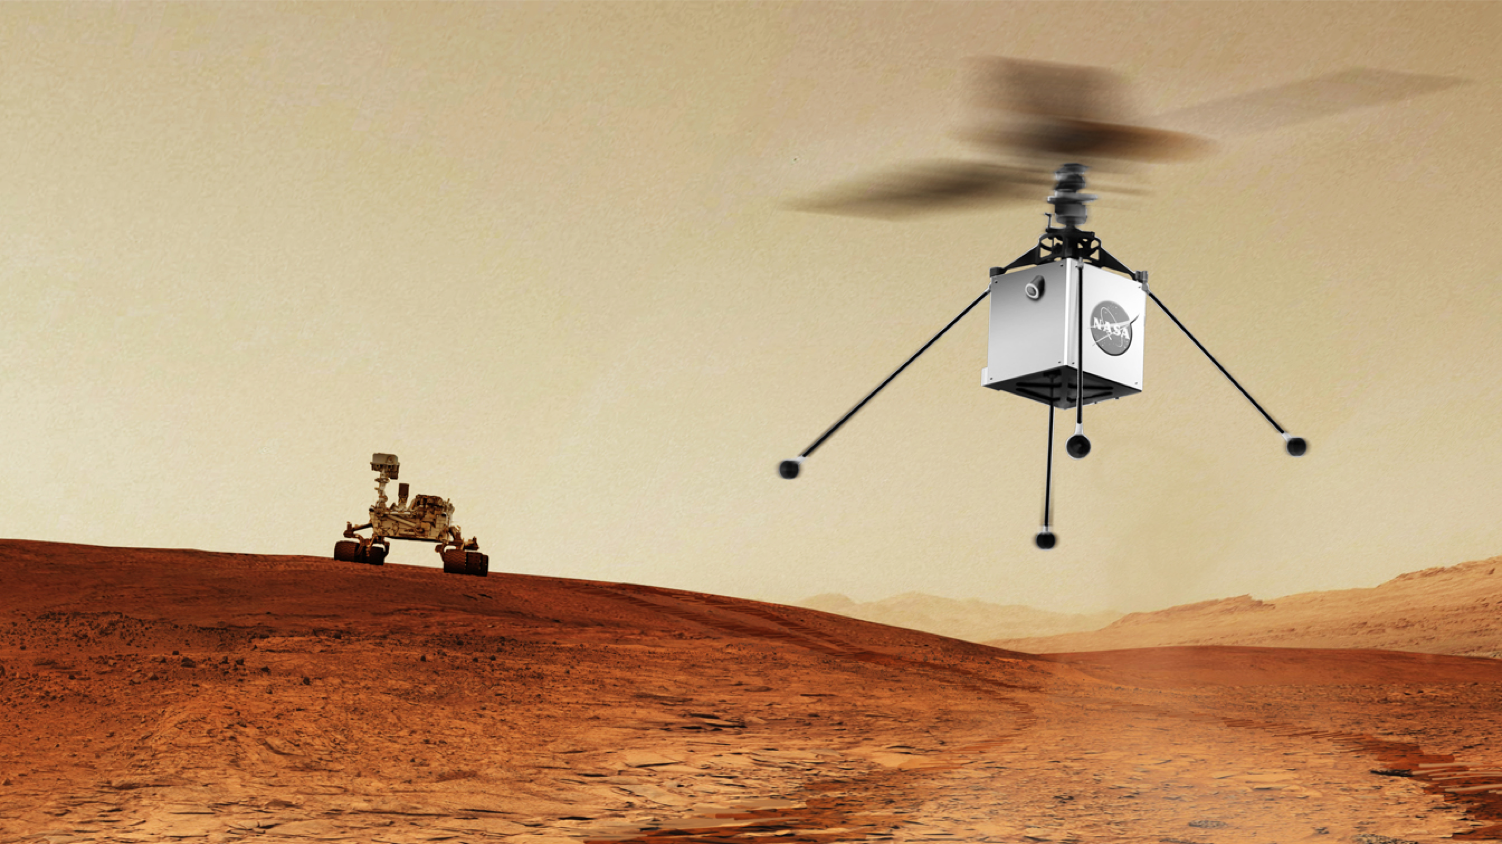
\includegraphics[width=0.99\columnwidth]{figs/heli-rover.png}
		\caption{Mars rover and Mars helicopter coordinating and navigating on unknown Mars terrains.}
		\label{fig:cover}
	\end{figure}
	
    %%%%%%%%%%%%%%%%%%%%%%%%%%%%%%%%%%%%%%%%%%%%%%%%%
    %%%%%%%%%%%%%%%%%%%%%%%%%%%%%%%%%%%%%%%%%%%%%%%%%
	\subsection{Highlights and contributions}
	The highlights and contributions of this work can be listed as follows.
	\begin{enumerate}
	
	{\color{orange}
	% contribution: system model and mars mission spec
	\item We rely on formal methods that can deal with stochastic partially observable systems, and we define complex specification for a two-robot team (i.e., rover, copter) in planetary exploration applications. In particular, we focus on complex missions that require rover and helicopter coordination, where the resulting formulae capture properties that take into account uncertainty
	over the robots' poses, and map (elevation, regions and their labels, presence of samples).
	
	%we can define constraints over the probability distribution of robot poses and the environment map.
	%The proposed method extends the formal methods to stochastic partially observable systems, where we can incorporate map uncertainty into the planning.
	%For example, we can express predicates like: the uncertainty of a given part of map needs to be less than a certain threshold.
	
	%\item We propose a framework to formally specify scientific exploration missions for a pair of copter and rover. Moreover, we consider and encode using \DTL a fragment of real mission specifications that the team must accomplish.
	
	
	% contribution: planning framework, where the two robots interact
	\item We propose a method that can handle failures and unexpected contingencies during the execution via re-planning or re-mapping the environment to get more information. The re-mapping phase is an instance of active perception behaviors that emerges of the proposed framework.
	
	\item We consider an interacting team of robots (copter and vehicle) and
	propose a framework that integrates on-line execution policy with active
	perception to detect perception failures/mismatches, on demand mapping of
	the environment by the copter when the currently available map is insufficient,
	dynamic re-planning in case of failure or remapping.
	
	% contribution: sampling-based algorithm for the rover
	\item We propose a sampling-based framework to synthesize 
	correct-by-construction policies for the rover that plans over maps provided
	the copter, where the map information can be extended on-demand.
	
	% contribution: case studies
	\item We highlight the proposed algorithms in two case studies involving
	space exploration missions for a rover-copter team.
	A simple case study is used to show the main features of the framework.
	The second example considers a real location on Mars that the robot team
	needs to explore.
	}
	
	% problem: we don't define a new logic, and the extension is rather thin. It is much better to focus on how we use DTL in the Mars mission case. See first contribution.
	\item The proposed method extends the formal methods to stochastic partially observable systems, where we can incorporate map uncertainty into the planning. For example, we can express predicates like: the uncertainty of a given part of map needs to be below a certain threshold.
	
	% problem: unclear what the contribution is from this paragraph. I re-focused it on a framework of interacting robots, and active perception is integrated in it.
	\item This framework results in active perception and information gathering behaviors. For example, to satisfy safety constraints, the system actively steers its sensors to gather more information about the parts of map that violate the safety constraints.
	
	% problem: this is not quite a contribution, it is already present in previous work
	\item The proposed method can express predicates directly over the system belief, rather than system state.
	
	% problem: this is good, but the feedback I usually receive from PIs is that contributions must be very crisp, i.e., stated very clearly. I integrated this into the second contribution above.
	\item The proposed method also handles execution failures. When things don't go according to plan during execution, the propose method re-plans or re-maps the environment to get more information.
	
	% problem: there is a wording problem. We didn't extend formal methods to space problems (see work by Brian Williams), but we applied it there. We can claim that we focus on rover space missions. See first and forth contribution.
	\item We extend the application of formal methods to space problems, in particular surface exploration via a two-agent system.
	\end{enumerate}
	
	%%%%%%%%%%%%%%%%%%%%%%%%%%%%%%%%%%%%%%%%%%%%%%%%%%%%%%%%%%%%%%%%%%%%%%%%
	\subsection{Related Work}
	\cristi{TODO: related work on
	(a) sampling-based methods for stochastic systems,}
	\cristi{(b) formal-methods in robotics in general,}
	The use of formal methods to specify mission goals for robot tasks has been successfully employed by \cite{DiKlChBe-RAM-2011,KB-TAC08-LTLCon}.  % Add citation to some of the work on language guided synthesis for scLTL and how it is related to solving reachability problems over automatons?
	\cristi{(c) emphasis on synthesis for stochastic systems with TL specs,}
    For finite state Markov decision processes properties expressed in PCTL and CSL can be verified by tools such as \cite{KNP11} and  \cite{dehnert2017storm}. 
	For Markov processes over uncountable state spaces, most results deal with  probabilistic evaluations of temporal logic specifications (PLTL) that can be formulated as automata specifications. By reformulation the formal verification and synthesis problem to a probabilistic reachability problem over the product between the original stochastic model and a deterministic finite-state automaton %, representing the specification,
	as introduced in \cite{AbateQuanti}, \cite{tmka2013} has shown that controlled discrete-time Markov Processes can be formally verified. Still, its  computational implementation  hinges on formal abstraction of the stochastic system to a finite state Markov decision chain \cite{soudjani2015faust}.  
	
		% In this paragraph, the formal methods are given for partially observable systems.
	For the safety verification of partially observable systems, \cite{Lesser2015} uses finite state approximations of stochastic hybrid systems to solve the safety problem over an equivalent information space. Next to the partial observations, also the knowledge that the system has been safe up to that moment is used to compute the belief space. % or sufficient statistic.
	In \cite{Cristi-CDC-2016}, the standard linear-time temporal logic has been extended to incorporate beliefs and uncertainty. 
	
	
	
	\cristi{	(d) closest work and how it differs (i.e., CDC/ISER papers, Austin's and Kevin's work).
	}

	
% 	In this section, we overview the most related work.
	
	In the last few years, formal methods has been extended to stochastic partially observable setting (e.g., \cite{Cristi-CDC-2016}, \cite{dorsa-rss2016}, \cite{fu2015integrating}). While these literature advance the formal methods approaches to partially observable and stochastic setting, there is a need for methods that enable replanning when the system faces with unmodeled contingencies. In other words, there exist a gap between planning and execution when it comes to real-world setup when the modelling assumption can be violated. Further, the uncertainty in the map has not yet been included in formal method approaches as a decision making parameter. In our application, the map uncertainty is a crucial factor in deciding what path is optimal and how/where the system need to increase its information to provide higher level of mission accomplishment success.
	
	%%%%%%%%%%%%%%%%%%%%%%%%%%%%%%%%%%%%%%%%%%%%%%%%%%%%%%%%%%
	\section{Belief Space Temporal Logic}
    {\color{red} [There is currently no problem definition, would it make sense to add this to the end of this section?]}
    
	In this section, we define a language for planning under uncertainty in partially-observable environments using formal methods. We will start by reviewing partially-observable systems and the POMDP problem. Then we will go over the belief-based temporal logic for mission planning.
	
    %%%%%%%%%%%%%%%%%%%%%%%%%%%%%%%%%%%%%%%%%%%%%%%%%%%%%%%%%%
	\subsection{POMDP}\label{sec:POMDP}
	Let us denote the system state, action, and observation at the $k$-th time-step by $x_k, u_k, z_k$, respectively. Let $x_{k+1}=f(x_k,u_k,w_k)$ and $z_k=h(x_k,v_k)$ denote the system dynamics and measurement models, where $w_k\sim p_w(\cdot|x_k)$ and $v_k\sim p_v(\cdot|x_k)$ denote the state-dependent process and observation noise. Due to the observation noise, the best one can infer about the system state is a probability distribution over all possible states, referred to as belief $b_k=p(x_k|z_{0:k})$. Belief space (i.e., the set of all beliefs) is denoted by $\mathbb{B}$. Belief is typically evolved using a recursive filter denoted by $\tau$ as $b_{k+1}=\tau(b_k,u_k,z_{k+1})$.
    {\color{red} In this work, we require that the belief space is a Polish space\footnote{With Euclidean spaces as a typical example a Polish space is a separable and completely metrizable topological space. } and that the recursive filter is a Borel measurable mappings.}
% * <haesaert@caltech.edu> 2017-10-31T06:56:01.319Z:
%
% > In this work, we require that the belief space is a Polish space\footnote{With Euclidean spaces as a typical example a Polish space is a separable and completely metrizable topological space. } and that the recursive filter is a Borel measurable mappings.
%
% ^.
    The control policy $\pi$ in a partially observable setting is a mapping from belief space to the action space, i.e., $u_k=\pi(b_k)$. Defining the one-step cost of taking action $u$ at belief $b$ by $c(b,u)$, we can formally define the POMDP problem as: 
    \begin{align}
    \pi^*=\arg\min_\pi\mathbb{E}\sum_{k=0}^{\infty}c(b_k,\pi(b_k))
    \end{align}
    Note that $c(b,u)=0$ for all $b\in B_{goal}$ and $c(b,u)>0$, otherwise. In this work, we aim to approximate and solve this problem while we satisfy mission specifications.
    
    
	\begin{figure*}[t!]
    	\centering
    % 	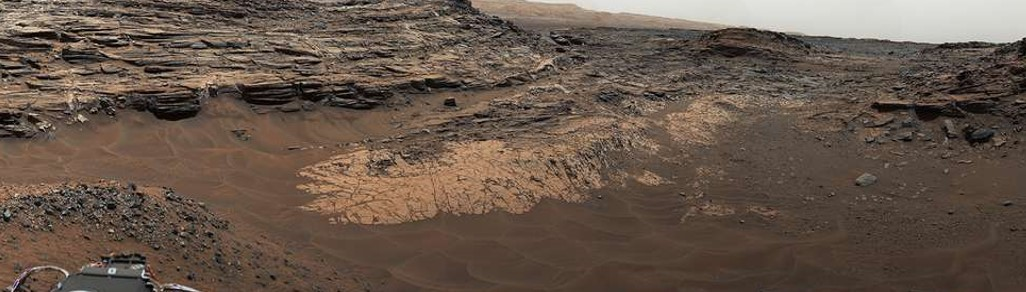
\includegraphics[width=1.4\columnwidth]{figs/map.png}
    	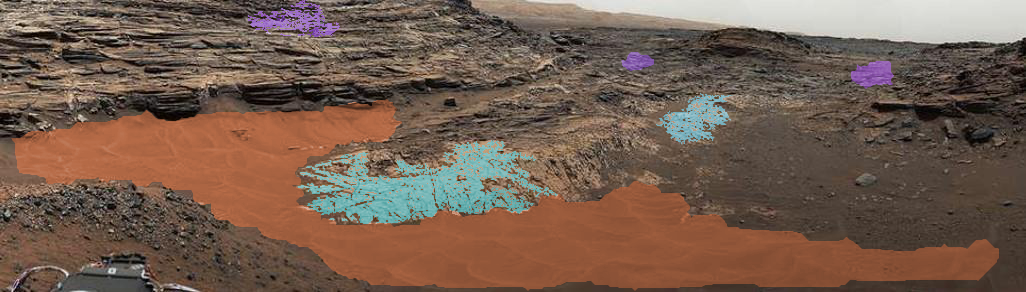
\includegraphics[width=2\columnwidth]{figs/MarsLabelledWithSand.png}
    	\caption{Labelled map of a typical campaign where blue and purple areas show regions containing science targets for the rover and orange area shows the region in sand.}
    	\label{fig:Scenario}
    \end{figure*}
    
    %%%%%%%%%%%%%%%%%%%%%%%%%%%%%%%%%%%%%%%%%%%%%%%%%%%%%%%%%%
	\subsection{\DTL}\label{sec:DTL}
    To encode mission specifications, and synthesize a controller to satisfy them, we resort to formal methods. To develop a language for formal planning and reasoning over the belief state, we rely on predicate-based logic.
    %\pr{Predicate-based logic vs. propositions-based logic}
    %In this work, we will rely on predicate logic because we explicitly reason about the belief of the system (e.g. covariance matrix) as opposed to proposition-based logic where the state of system is implicit in the definitions of the propositions.
    
    %a predicate temporal logic defined over the space of Gaussian distributions with fixed dimension.
    
    \pr{Notation}
    Let $\Sigma$ be a finite set. The cardinality,
    power set, Kleene- and $\omega$-closures
    of $\Sigma$ are denoted by $\card{\Sigma}$,
    $\spow{\Sigma}$, $\Sigma^*$ and $\Sigma^\omega$,
    respectively.
    $A \subseteq \BB{R}^n$ and $B \subseteq \BB{R}^m$,
    $n, m \geq 0$, we denote by $\CA{M}(A, B)$ the set of
    functions with domain $A$ and co-domain $B$, where $A$ has positive measure with
    respect to the Lebesgue measure of $\BB{R}^n$.
    The set of all positive semi-definite matrices of size
    $n \times n$, $n \geq 1$, is denoted by $S^n$.
    $\BB{E}[\cdot]$ is the expectation operator.
    The $m \times n$ zero matrix and
    the $n \times n$ identity matrix are denoted by
    $\BF{0}_{m, n}$ and $\BF{I}_n$, respectively.
    The supremum and Euclidean norms are denoted by
    $\norminf{\cdot}$ and $\normeucl{\cdot}$, respectively.
    
    \pr{Parametrized Belief space}
    In this work, we assume that the belief space $\mathbb{B}$ is  a finite dimensional space and that it can be parameterized. For example, let $\CA{G}$ denote the Gaussian belief space
    of dimension $n$, i.e. the space of Gaussian
    probability measures over $\BB{R}^n$.
    For brevity, we identify the Gaussian measures
    with their finite parametrization, mean and
    covariance matrix. Thus,
    $\CA{G} =  \BB{R}^n \times  S^n$.
    If $\BF{b} = b^0b^1 \ldots \in \CA{G}^{\omega}$,
    we denote the suffix sequence $b^i b^{i+1} \ldots$ by
    $\BF{b}^i$, $i \geq 0$. Each member of $\Sigma^*$ and $\Sigma^\omega$ is referred to as ``word" or "sequence". 
    
    For the language grammar we will rely on Bakus-Naur form. $\True$ and $\False$ are Boolean constants that respectively describe specifications that are always satisfied or can never be satisfied. 
    Predicate $f\leq 0$ is defined as a Borel measurable function $f:\mathbb{B}\rightarrow \mathbb{R}$ that encodes constraints or properties over belief space. Defining predicates over the belief space allows us to enforce properties directly on the probability distribution of the system (and hence its chance constraints). Some examples are \textbf{(i)} Bounds on determinant or trace of of the covariance matrix (i.e., $det(P)$, $Tr(P)$) to  bound the uncertainty about the system's state. \textbf{(ii)} Bound on projection of covariance matrix $\Pi P$ to bound the uncertainty in a specific direction.
% * <haesaert@caltech.edu> 2017-10-31T06:59:20.048Z:
%
% >  Bakus-Naur form. 
%
% ^.
    \textbf{(iii)} Bounds on state mean $\hat{x}$ to specify
    where in the state space the system should be. \textbf{(iv)} Bounds on Mahalanobis distance $\mathcal{M}(\hat{x},P,x) = (\hat{x}-x)^TP^{-1}(\hat{x}-x)$.
    to describe the distance from a point to a Gaussian distribution, when specifying a desired state (or region) in the state space. We then combine these predicates via operators to create specifications. Operators include boolean "and" $\andltl$, "or" $\orltl$, "not" $\notltl$, and temporal operators: "until" $\Until$, "eventually" $\Event$, "always" $\Always$, "next" $\Next$.
    
    %\pr{Structure of the formulae}
    %Parts of the formulae is not part of the syntax but rather ... In particular $|$ defines option. For example, $\phi::=A | B$ means specification $\phi$ can be either $A$ or $B$. Example: an arithmetic expression has the following syntax grammar $expr::= c | x | expr + expr | expr - expr | expr * expr | expr / expr$.
    
    \begin{definition}[\DTL Syntax]
    \label{def:gdtl-syntax}
    The {\em syntax} of \DTL includes the minimum number of operators to define the logic:
    \begin{equation*}
     \phi :=  \True \ |\ f \leq 0 \ |\ \notltl \phi \ |\ \phi_1 \andltl \phi_2 \ |\ \phi_1 \Until \phi_2 \ |\ \Next \phi
    \end{equation*}
    %where $\True$ is the Boolean constant ``True'',
    %$f \leq 0$ is a predicate over $\mathbb{B}$, where
    %$f \in \CA{M}(\mathbb{B}, \BB{R})$.
    %$\notltl$ is negation (``Not''), $\andltl$ is conjunction (``And''),
    %$\Next$ is ``Next'',
    %and $\Until$ is ``Until''.
    \end{definition}

    For convenience, we define the additional operators:
    $\phi_1 \orltl \phi_2 \equiv  \notltl (\notltl \phi_1 \andltl \notltl \phi_2)$,
    $\Event \phi \equiv \True \Until \phi$, and
    $\Always \phi \equiv \notltl \Event \notltl \phi$,
    %\begin{align*}
    %\phi_1 \orltl \phi_2 & \equiv  \notltl (\notltl \phi_1 \andltl \notltl \phi_2) \\
    %\LTLEVENTUALLY \phi & \equiv \True \LTLUNTIL \phi \\
    %\LTLALWAYS \phi & \equiv \notltl \LTLEVENTUALLY \notltl \phi
    %\end{align*}
    where $\equiv$ denotes semantic equivalence. \DTL syntax defines the symbols and their correct ordering to form a formulae. In the following, we define \DTL semantics, i.e., the meaning of those symbols.

    \begin{definition}[\DTL Semantics]
    \label{def:gdtl-semantics}
    Let $\BF{b} = b^0b^1 \ldots \in \mathbb{B}^{\omega}$
    be an infinite sequence of belief states. $\BF{b} \models \phi$ denotes the event that the word $\BF{b}$ satisfies specification $\phi$. Accordingly, the {\em semantics} of \DTL is defined recursively as
    \begin{align*}
    &\BF{b}^i \models  \top  & \\
    &\BF{b}^i \models f \leq 0 & \Equiv\quad & f(b^i) \leq 0\\ % \forall (x,P) \in b^i \\
    &\BF{b}^i \models \notltl \phi & \Equiv\quad & \notltl (\BF{b}^i \models \phi) \\
    &\BF{b}^i \models \phi_1 \andltl  \phi_2  & \Equiv\quad & ( \BF{b}^i \models \phi_1 ) \andltl ( \BF{b}^i \models \phi_2 ) \\
    &\BF{b}^i \models \phi_1 \orltl  \phi_2  & \Equiv\quad & ( \BF{b}^i \models \phi_1 ) \orltl ( \BF{b}^i \models \phi_2 ) \\
    &\BF{b}^i \models  \phi_1 \Until \phi_2 & \Equiv\quad & \exists j \geq i \text{ s.t. } ( \BF{b}^j \models \phi_2 ) \\
    & & & \andltl (\BF{b}^k \models \phi_1, \forall k \in \{i, \ldots j-1\})\\
    &\BF{b}^i \models \Event \phi  & \Equiv\quad & \exists j \geq i \text{ s.t. } \BF{b}^j \models \phi \\
    &\BF{b}^i \models \Always \phi  & \Equiv\quad & \forall j \geq i \text{ s.t. } \BF{b}^j \models \phi
    \end{align*}
    
    \end{definition}
    
% 	\begin{figure}[h!]
% 		%\vspace*{-20pt}
% 		\centering
% 		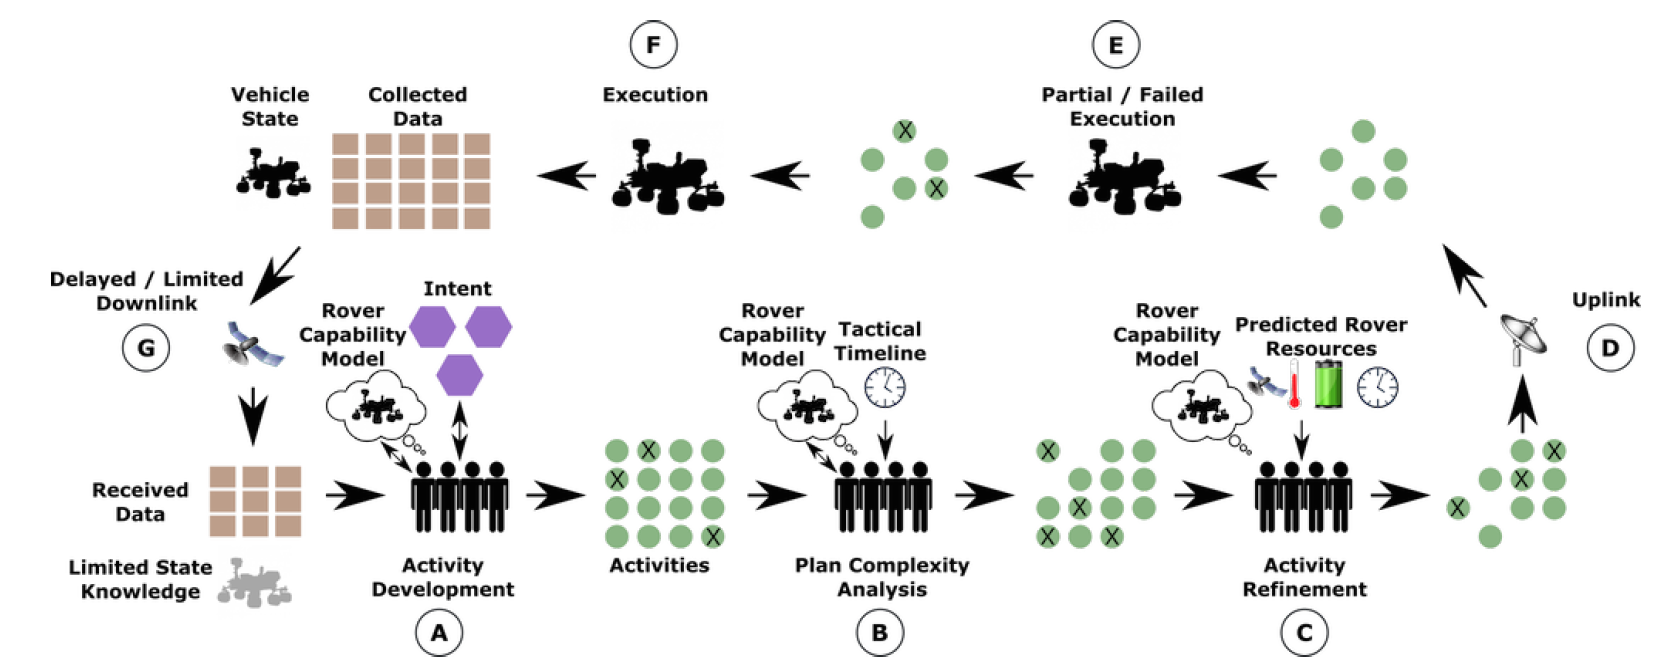
\includegraphics[width=0.8\columnwidth]{figs/HumanInLoop.png}
% 		\caption{Typical inverse sensor model for a range sensor. It returns the occupancy probability for voxels on the measurement ray/cone based on their distance to the camera.}
% 		\label{fig:invSensorModel}
% 	\end{figure}
	
	%%%%%%%%%%%%%%%%%%%%%%%%%%%%%%%%%%%%%%%%%%%%%%%%%%%%%%%%%%%%%%%%%%%%%%%%
	\section{Illustrative science campaign}
	Existing Mars rover (and future Mars copter) missions are prescribed via science campaigns. Each campaign is comprised of many science goals and mission requirements. In this section, we present a science campaigns that we have selected for Mars helicopter and Mars Rover coordination and navigation scenario. Fig. \ref{fig:Scenario} shows a map of the ?? area on Mars surface created by ?? [?]. To describe the science campaign, we start by listing a set of requirements for typical Mars missions. These requirements are generated by rover planers and systems engineers at JPL. Then, we show how to model these requirements using the \DTL language.
    
    %%%%%%%%%%%%%%%%%%%%%%%%%%%%%%%%%%%%%%%%%%%%%%%%%%%%%%%%%%%%%%%%%%%%%%%%
	\subsection{Mission specification}
	\label{sec:misspec}
	Below is a set of requirements that specifies a science campaign.
	\begin{enumerate}
      \item \textit{Rover must visit any two of the science targets type A and one of the science targets type B}. These areas are shown in purple and blue, respectively, in Fig. \ref{fig:Scenario}. They represent areas for potentially high-science-value rock/soil samples that need to be collected.
      \item \textit{Rover must maintain the variance of its state below $\Sigma_{max}$}. This specification is to maintain accuracy along the mission and reduce the risk of unexpected events.
      \item \textit{Rover routes must avoid hazards}. These hazard areas represent large rocks, deep sands, steep slopes, etc, which are given as the regions labeled on the map as part of the science campaign.
      \item \textit{Rover must follow speed constraints}. Fig. \ref{fig:SpeedConstriants} encodes the speed constraints. Rover's maximum speed is a function of cumulative fractional area [?] and the terrain slope.
      \item \textit{Copter and Rover must satisfy battery and power constraints}. In particular, Mars helicopter can only fly for 2-3 minutes per day. Thus, at each stage, the remaining battery level plays an important role in shaping the mission.
      \item \textit{Mars copter must avoid landing near hazards}. These hazards include large rocks, deep sands, steep slopes, etc.
      \item \textit{Copter must maintain a minimum distance $d_{min}$ and a maximum distance $d_{max}$ from the rover}. This specification is because the main asset of the this mission is rover as it carries all important science instruments. Therefore the copter should not pose any risk for the rover, in case of copter failure.
    \end{enumerate}

    \begin{figure}[h]
	\centering
	%\subimport*{figs/}{graph.tex}	
	\scalebox{.5}{\documentclass{standalone}
\usepackage{tikz}
\usetikzlibrary{calc,arrows}
\usepackage{verbatim}
\usepackage{pgfplots}
\usepackage{gensymb}
\usetikzlibrary{positioning}

% argument #1: any options
\newenvironment{customlegend}[1][]{%
    \begingroup
    % inits/clears the lists (which might be populated from previous
    % axes):
    \csname pgfplots@init@cleared@structures\endcsname
    \pgfplotsset{#1}%
}{%
    % draws the legend:
    \csname pgfplots@createlegend\endcsname
    \endgroup
}%
% makes \addlegendimage available (typically only available within an
% axis environment):
\def\addlegendimage{\csname pgfplots@addlegendimage\endcsname}

\pgfplotsset{compat=1.15}
\begin{document}

\tikzset{font={\fontsize{15pt}{15}\selectfont}}
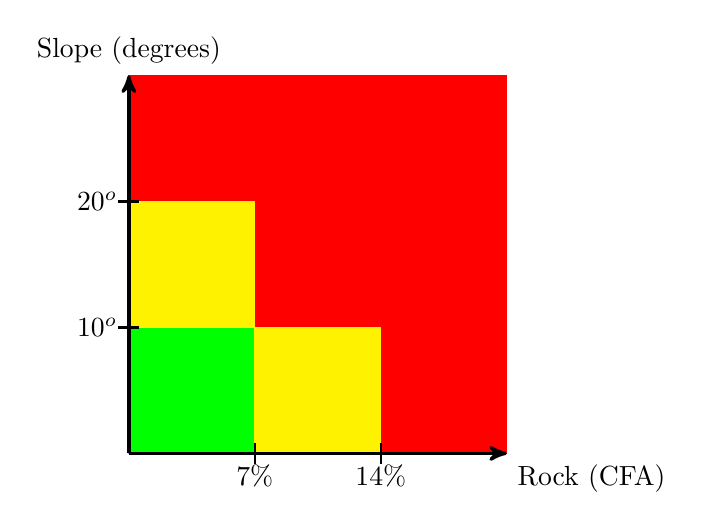
\begin{tikzpicture}[
        %We set the scale and define some styles
        scale=1.5,
        axis/.style={very thick, ->, >=stealth'},
        important line/.style={thick},
        dashed line/.style={dashed, thick},
        every node/.style={color=black}
    ]
    % Important coordinates are defined
    \newcommand\x{3.2}

    %We make some nice shading to annotate different parts of the curve
    %  Stop
    \draw [fill=red,red] (0,0) rectangle (\x,\x);
    
    % High Speed
    \begin{scope}
    \draw [fill=green,green] (0,0) rectangle (\x/3,\x/3);
    \end{scope}
    % Low Speed
    \begin{scope}
    \draw [fill=yellow,yellow] (0,\x/3) rectangle (\x/3,2*\x/3);
    \draw [fill=yellow,yellow] (\x/3,0) rectangle (2*\x/3,\x/3);
    \end{scope}
    % Axis
    \begin{scope}
    \draw[axis] (0,0)  -- (\x,0) node(xline)[below right]{Rock (CFA)};
    \draw[axis] (0,0) -- (0,\x) node(yline)[above]{Slope (degrees)};
    \end{scope}
    % Cordinates
    \draw[thick] (\x/3,-2.5pt) -- (\x/3,2.5pt) node[below=0.15] {7\%};
    \draw[thick] (2*\x/3,-2.5pt) -- (2*\x/3,2.5pt) node[below=0.15] {14\%};
    \draw[thick] (-2.5pt,\x/3) -- (2.5pt,\x/3) node[left=0.15] {10$^{o}$};
    \draw[thick] (-2.5pt,2*\x/3) -- (2.5pt,2*\x/3) node[left=0.15] {20$^{o}$};
    
    % \begin{customlegend}[
    % legend entries={High Speed, Low Speed, Stop},
    % legend style={at={(\x,\x)}, font={\fontsize{7pt}{7}\selectfont}}]
    % % the following are the "images" and numbers in the legend
    % \addlegendimage{area legend,green,fill=green}
    % \addlegendimage{area legend,yellow,fill=yellow}
    % \addlegendimage{area legend,red,fill=red}
    % \end{customlegend}
\end{tikzpicture}
\end{document}}
	\caption{Speed Constraints for Slope vs Rock CFA (Cumulative Fractional Area). High speed (green), Low speed (yellow) and Stop (red).}
	\label{fig:SpeedConstriants}
    \end{figure}

    %%%%%%%%%%%%%%%%%%%%%%%%%%%%%%%%%%%%%%%%%%%%%%%%%%%%%%%%%%%%%%%%%%%%%%%%
	\subsection{Example Mission Execution}
	In this section, we describe an example instance of the functional architecture shown in Fig. \ref{fig:FuncArc}, that may occur during the execution of the campaign. 
	
	We start the campaign by flying the helicopter in the environment and generating a labelled map that classifies science targets, cumulative fraction area (CFA) covered by rock and hazardous regions. During this time, the helicopter maintains the constraints on battery level, distance from the rover and avoids terrain hazards while landing. The rover gets the labelled map from the helicopter and mission requirements from users on Earth. Using this, the rover computes a control policy and executes it to move along a desired path in the environment.
	
	During execution, the rover detects non-traversibility, eg. excessive slip due to large slope or larger CFA that was not accurately estimated in the labelled map obtained from the helicopter. Now, the rover updates the correct labels in map and tries to recompute the policy. If it is not possible to find a feasible policy that satisfies all the mission requirements, it asks the copter to fly and re-map the unexplored regions. On getting the information of the unexplored regions, it recomputes a control policy and resumes execution.
% 	\begin{enumerate}
% 	\item Copter maps the environment and generates a labelled map to classify science targets, rock CFA, slope and hazardous regions.
% 	\item copter sends the map to rover 
% 	\item rover selects a path
% 	\item rover follows the path
% 	\item rover detects non-traversability (e.g., excessive slip)
% 	\item rover decides to replan
% 	\item rover find a new path
% 	\item the new path goes through an area of map that is not well mapped
% 	\item rover asks copter for further map information
% 	\item copter looks at its resources, wind,  terrain conditions, and it is distance from the rover
% 	\item copter realizes that it has enough resources to help the rover by generating a more detailed map
% 	\item copter goes to the target area and maps it
% 	\item copter sends the new map to the rover
% 	\item rover follows the new path happily!
% 	\item copter lands at a spot happily to recharge for tomorrow's mission
% 	\end{enumerate}
    	\begin{figure}[h!]
    	\centering
    	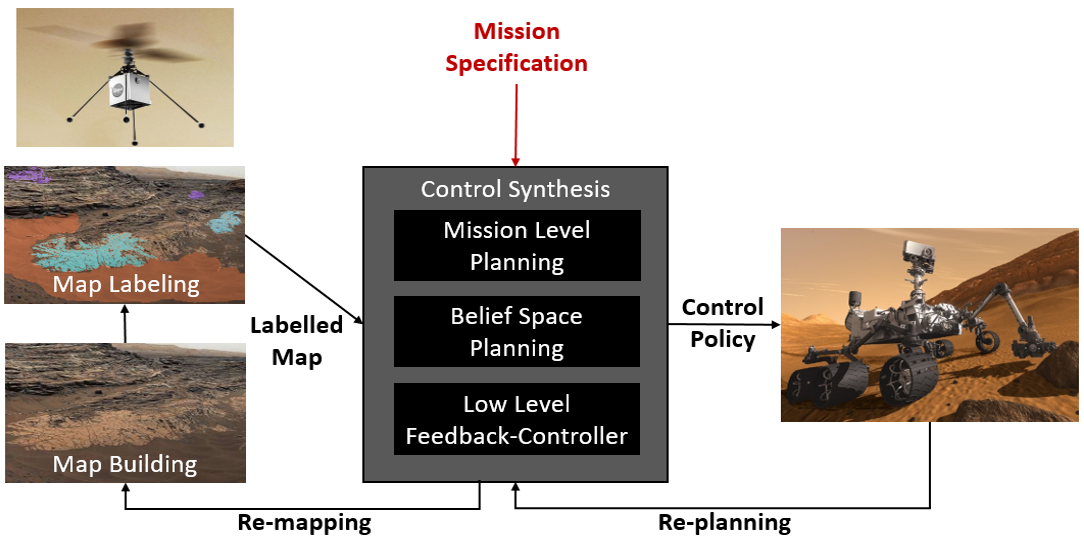
\includegraphics[width=\columnwidth]{figs/FunctionalArcV3.png}
    	\caption{Functional Architecture.}
    	\label{fig:FuncArc}
    \end{figure}
	


%     copter mapping generates $b(m|z_{0:k})$
%     \begin{align}
% 	m_k^{ml} = \arg\max_m b(m|z_{0:k})
% 	\end{align}
% 	$var(b(m^{i}|z_{0:k}))>threshold$
	
	%%%%%%%%%%%%%%%%%%%%%%%%%%%%%%%%%%%%%%%%%%%%%%%%%%%%%%%%%%%%%%%%%%%%%%%%
	\subsection{System Model}\label{sec:SysModel}
    To translate the specification to mathematical predicates, we start by defining the system state and belief. Note that in this section, we are proposing a general formulation of the problem with belief over rover, copter and map. However, for the simulation in section \ref{sec:simulation} we focus on the planning and execution problem of the rover and assume a deterministic map and deterministic copter dynamics.
    
    Our system described by state $x$ is comprised of a rover $x^r$, a copter $x^c$, and the environment $m$.
    \begin{align}
        x = (x^r, x^c, m) 
    \end{align}
    Due to the noise in system motion and perception, the best one can infer about the system state is its belief, i.e., the probability distribution over all possible states, denoted by $b_k=p(x|z_{0:k})$. In this work, we approximate the joint belief over rover, copter, and the environment, with three separate marginalized beliefs.
    \begin{align}
        \nonumber
        b_k &= p(x|z_{0:k})=p(x^r, x^c, m|z_{0:k})\\
        &\approx p(x^r|z_{0:k})p(x^c|z_{0:k})p(m|z_{0:k})=:(b^r, b^c, b^m)
    \end{align}
    The above assumption means that, in the control synthesis layer, we are not solving the full SLAM problem, and rather we are treating the localization and mapping problems separately. %It is worth noting that the SLAM 
    
    % \begin{align}
    %     b \equiv (\hat{x}^r, \hat{x}^r, P, b^{m})
    % \end{align}
    %where
    The robot state $x^r=(p^r, v^r, q^r)$ is comprised of the rover pose $p^r$, rover velocity $v^r$, and rover battery charge level $q^r \in [0, 1]$. Similarly, the copter state $x^c=(p^c, v^c, q^c)$ includes pose, velocity, and charge level of the copter. We represent the belief over rover and copter state by Gaussian, characterized by its mean and covariance $b^r\equiv(\hat{x}^r,P^r)$, $b^c\equiv(\hat{x}^c,P^c)$. 
    To describe the map, we follow the traditional occupancy grid map representation, where map is comprised of voxels $m=(m^1,\cdots,m^n)$. Each voxel contain the terrain height $h^i$ and terrain type $l^i$ at that voxel, i.e., $m^i = (h^i,l^i)$. We have a set $L$ of predefined terrain labels, such as rock, deep sample, steep slopes, unseen areas, etc. Note that $l^i$ can take belong to multiple labels. We represent this fuzzy belonging via a label belief $b^{l^i}:L\rightarrow[0,1]$, i.e., $b^{l^i}$ will assign a probability for voxel $i$ to belong to each given label. We assume that the belief over height and type are independent $b^{m^i} = b^{h^i}\times b^{l^i}$. 
    
    %The belief over height is $b^{h^i}=p(h^i|z_{0:k)}$ and the belief over terrain label is $b^{l^i}=p(l^i|z_{0:k})$.
    
    %%%%%%%%%%%%%%%%%%%%%%%%%%%%%%%%%%%%%%%%%%
    \subsection{Mission specification in \DTL}
    \label{sec:gdtlspec}
    In this section, we define the \DTL predicates corresponding to the mission specifications described in Section~\ref{sec:misspec}.
    
    We start by defining the overall specification (i.e., $\phi$) for the campaign in hand:
    \begin{align}\label{eq:overallspec}
        \phi = \phi_{science} \land \Always (\pred_{uncert} \land \phi_{safety} \land \phi_{dynamic})
        % \Until \pred_{complete},
    \end{align}
    which expresses the mission where the science objective $\phi_{science}$ needs to be satisfied and we always need to maintain a desired level of accuracy (expressed by $\zeta_{uncert}$, safety $\phi_{safety}$, and dynamics constraints $\phi_{dynamic}$.
   \sofie{[See later comment on this.]}

\noindent\pr{Science} The science objective in this campaign is to collect two samples from high-valued science areas A and one sample from area B. Let $\pred_{X} = p^r \in X$ denote the event that pick up a sample from region $X$ that is subset of the terrain.
    \begin{align}
        \phi_{science} = \Event ((\pred_A \land \pred_{\exists A}) \land
        \Event (\pred_A \land \pred_{\exists A})) \land
        \Event (\pred_B \land \pred_{\exists B})
    \end{align}
    where $\pred_{\exists X}$ refers to the event that there exist a desired sample to pick up at region $X$.
    \begin{align}
    \pred_{\exists X} = \sum_{m^i \subseteq X} p(l^i=X) \geq \epsilon_{sc}\geq 0
    % \int_X \int_{\Real^2} m^i(x) K(x | p) \df x \df p \geq \epsilon_{sc}\geq 0
    \end{align}
    \pr{Uncertainty} The uncertainty objective is to maintain the desired level of accuracy on their estimated state (e.g., robots need to know where they are with respect samples) during the mission. 
    \begin{align}
        \nonumber\pred_{uncert} = tr(P^r) < \Sigma^r_{max}\\
        \pred_{uncert} = tr(P^c) < \Sigma^c_{max}
    \end{align}
    
   \noindent \pr{Safety specification} Space application falls into the category of safety-critical applications. Thus, maintaining the safety of systems along the operation is a very important objective of the mission. We express the safety specification as:
	\begin{align}
	   \phi_{safety} &= \phi_{keepout} \land \pred_{near} \land \phi_{charge}
	\end{align}
	In the following paragraphs, we will explain each term in the definition of above safety specification.
	
	\noindent\pr{Keep-out predicate}
	$\phi_{keepout}$ encodes the distance from risky regions of the map such as non-traversable obstacles, sandy areas with a risk of getting stuck, cliffs, high-slope areas, etc. We will define keep-out constraints for both rover and copter.
	\begin{align}
	   %\phi_{keepout} &= \bigwedge_{o\in O} (\pred_{keepout}^r \land \pred_{keepout}^c)
	   \phi_{keepout} &= \bigwedge_{o\in O} (\pred_{keepout}^r \land (\pred_{keepout}^c \lor h^c > \epsilon_{h}^c))
	\end{align}
	where risk areas are extracted from the map $m^t$ based on the labels. Each risk region is approximated by Gaussian distribution $o \sim\mathcal{N}(\hat{p}^o, P^o)$, in which $\hat{p}^o$ represents the mean of the risk area and $P^o$ is the spatial variance of the risk area. For obstacle $o$, rover's keepout specification can be written as:
	\begin{align}
    	\pred_{keepout}^r = (\hat{p}^r-\hat{p}^o)^T(P^r+P^o)^{-1}(\hat{p}^r-\hat{p}^o) \geq \epsilon_{safety}^r
	\end{align}
	where $\hat{p}^r$ and $P^r$ are the position and associated uncertainty of the rover. For the copter, we have the same constraints when its height is below a threshold
	\begin{align}
    	\pred_{keepout}^c = (\hat{x}^c-\hat{x}^o)^T(P^c+P^o)^{-1}(\hat{x}^c-\hat{x}^o) \geq \epsilon_{safety}^c
	\end{align}
	where $\hat{p}^c$ and $P^c$ are the position and associated uncertainty of the copter.
    
\noindent\pr{Rover-copter distance predicate} In Mars copter/rover missions, rover is the mother-craft and the vital part of the mission, whereas the copter is a daughter-craft. Since the rover is carrying almost all science payload and instruments, the copter should not pose any risk to rover's functionality. Thus, copter has to always maintain a minimum distance from rover to avoid costly collisions with rover in the case of copter failure. Below specification expresses this mission requirement.
 	\begin{align}
 	    f_{coll} = \int b^{s}(x)\times b^{m}(x)dx - \epsilon_{coll} \\
 	    \pred_{near} = d_{min} \leq \norm{\overline{x}^r - \overline{x}^c} \leq d_{max}
 	\end{align}
    where $\overline{x}^r$ and $\overline{x}^c$ denotes the 2D position of the rover and copter, respectively, on the Mars surface.

\noindent\pr{Charge predicates} Energy is a critical issue in space missions. For a solar-powered rover and copter, and for each given campaign, $\zeta_{base}$ dxefines an area on Mars surface with a high-level of sun light intensity, where the vehicles can re-charge themselves. We express the charging constraint of both vehicles as:
 	\begin{align}
	    \phi_{charge} &= \phi_{charge}^r \land \phi_{charge}^c
	\end{align}
	where for each vehicle $s \in \{r, c\}$, we have
	\begin{align}
	    \phi_{charge}^s &= q^s \geq \epsilon_{battery}^s \Implies \Event (\xi^s_{Base} \Until q^s \geq \epsilon_{charged}^s)
	\end{align}
	Note that $\epsilon_{battery}^S$, for each vehicle is chosen large enough to permit return to the base.

\noindent\pr{Dynamics predicates} Due to rover and copter mechanical/electrical capabilities, these assets should not exceed certain velocity levels given the environment status. The following specification captures such mission requirements.
    \begin{align}
	    \phi_{dynamic} = \norm{v^r} \leq \epsilon_{velocity}^r(m)
	\end{align}
	where $\epsilon_{velocity}^r(m)$ is the velocity
	bound for the rover and copter, respectively, and depend on the map belief and position.
	Fig.~\ref{fig:SpeedConstriants} shows the dependence of the velocity with respect to
	map features (steep slopes, rocks).
	
% 	\pr{Mission completed predicate}
% 	\begin{align}
% 	    \phi_{complete} = c(A) \geq 2 \land c(B) \geq 1
% 	\end{align}

%    ------------------------------------------------------

% 	\begin{align}
% 	\phi = \phi_{reachGoal} \andltl \phi_{safety} \andltl \phi_{science}
% 	\end{align}
	
% 	\pr{Collision predicate}
% 	\begin{align}
% 	f_{coll}(b) = \int b^{s}(x)\times b^{m}(x)dx - \epsilon_{coll}
% 	\end{align}
% 	$b^s$ is the belief of the system (rover and copter)
	
	
% 	\pr{Charge predicate}
% 	\begin{align}
% 	f_{charge}(b) = b^{b}(x) - \epsilon_{battery}
% 	\end{align}
	
% 	\pr{Safety specification}
% 	\begin{align}
% 	\phi_{safety} = \Always (f_{coll}(b)\leq 0 \andltl f_{charge}(b) \leq 0 \andltl f_{keep-out}(b) \leq 0)
% 	\end{align}
	
% 	\pr{Keep-out predicate rover-single obstacle}
% 	\begin{align}
% 	f_{coll,rover}(b^r, b^o) = (\hat{x}^r-\hat{x}^o)^T(P^r+P^o)^{-1}(\hat{x}^r-\hat{x}^o)-\epsilon_{roverSafety}
% 	\end{align}
	
% 	\pr{Keep-out predicate copter-single obstacle}
% 	\begin{align}
% 	f_{coll,copter}(b^c, b^o) = (\hat{x}^c-\hat{x}^o)^T(P^r+P^o)^{-1}(\hat{x}^c-\hat{x}^o)-\epsilon_{copterSafety}
% 	\end{align}
	
% 	\begin{align}
% 	\phi_{keepout} = \andltl_{o\in O} (f_{coll,copter}(b^c, b^o)\leq 0 \andltl f_{coll,rover}(b^r, b^o)\leq 0)
% 	\end{align}
	
% 	what vs. how
	
% 	if rover safety in the next n steps is not satisfied, characterize which keepout zone vertex contributes the most... check safety gain versus energy consumption for copter... and then send the copter if it worth it... if not loop over all other vertices...
	
% 	\begin{align}
% 	\nonumber&\phi_{SafetyIncrease} =
% 	\Big(\andltl_{0\leq k\leq n} \Next^k \notltl (\phi_{keepout} \andltl f_{charge} \leq 0 \andltl f_{coll} \leq 0) \Big) \\
% 	&\Rightarrow \Big(\orltl_{v \in vertices} (IG(v)\geq \epsilon_{ig} \andltl f_{charge} \geq \epsilon_{ch} \Rightarrow \Event visit(b^c, v) ) \Big)
%     \end{align}
	
% 	we will use sub-formulae to write this in a hierarchical fashion... for example the second line above could specify the "active perception" subformulae.
	
	%%%%%%%%%%%%%%%%%%%%%%%%%%%%%%%%%%%%%%%%%%%%%%%%%%%%%%%%%%%%%%%%%%%%%%%%
% 	\section{Planning Problem Formulation} \label{subsec:problem}
% 	In this paper, ...
	
	
%%%%%%%%%%%%%%%%%%%%%%%%%%%%%%%%%%%%%%%%%%%%%%%%%%%%%%%%%%%%%%%%%%%%%%%%
\section{Control policy synthesis} \label{sec:planner}
In this section, we describe our approach to generate a control policy that drives the rover to the desired belief state $b^r_{des}$ while satisfying all the mission requirements specified in \DTL in Section \ref{sec:gdtlspec}. We start by converting the \DTL specifications to a Finite State Automaton (FSA), described in Section \ref{FSA}. Then we describe how sampling based methods in belief space are used to compute transition probabilities of FSA in Section \ref{sec:FIRM} and \ref{TransProb}. We then define the product \DTL-FIRM in Section \ref{DTL-FIRM}. Afterwards, we detail the procedure to find a policy that maximizes the probability of specification satisfaction. Section \ref{replanning} shows how we handle execution failures by re-planning and mapping the unexplored regions. Finally, in Section \ref{complexity}, we discuss the complexity of the proposed algorithm.

%Local controllers drive the systems along these paths and stabilize at key points. 
%The closed-loop behavior of the system induces paths in the belief space. 
%The FIRM describes the stochastic process that generates these paths. 
% We build an MDP by combing the FIRM with a Rabin automaton which then allows us
% to check if sample paths satisfy a GDTL formula. We
% compute transition probabilities and intersection probabilities
% (probability of intersecting a good or bad set from the Rabin
% automaton’s acceptance condition) for each edge in this
% structure.
% We use dynamic programming to find the policy
% in this structure that maximizes the probability of satisfying
% the formula. The resulting policy can then be translated to

%%%%%%%%%%%%%%%%%%%%%%%%%%%%%%%%%%%%%%%%%%%%%%%%%%%%%%%%%%%%%%%%%%%%%%%%
\subsection{Finite State Automaton}\label{FSA}
%\pr{GDTL to LTL conversion}
% FIRM graph introduced in Section \ref{sec:FIRM} captures the evolution of the system belief and in this section we discuss Rabin automaton that captures the evolution of the mission specification satisfaction.
We start by describing the process of converting the high level mission specifications expressed in \DTL into a Finite State Automaton (FSA) that captures the evolution of specification satisfaction. To generate the FSA, we first convert \DTL to LTL simply by converting the predicates to symbols~\cite{JonesDTL2013}, and then we use {\em spot}~\cite{duret14} to convert the LTL specifications to FSA.
% Symbol vs. predicates function
% $f\equiv f(b_k)\leq 0$
% $f\in F_\phi$
% $f(\cdot)\in F^{\cdot}_{\phi}$
Denoting the set of symbols that correspond to the predicates in \DTL formula $\phi$ as $F_\phi$, we formally define the FSA as follows:

%To check the presence of a belief trajectory that satisfies the mission specification, we rely on Rabin automoton that 
%Algorithm \ref{alg:compute-mdp} checks for the presence of a satisfying path in belief space using a deterministic Rabin automaton (DRA) $\RA$ that is computed from the GDTL specification using an intermediate linear temporal logic (LTL) construction~\cite{JonesDTL2013}.
%There exist efficient algorithms that translate LTL formulae into Rabin automata~\cite{klein2006}.

\begin{definition}[Finite State Machine]
A (deterministic) Finite State Machine is a tuple $\FSA = (S_\FSA, s_0^\FSA, \Sigma, \delta_\FSA, Acc_\FSA)$, where %:
$S_\FSA$ is a finite set of states, $s_0^\FSA \in S_\FSA$ is the initial state,
$\Sigma$ is the input alphabet with $\sigma\in\Sigma$ being a letter (or event) that triggers the transition between the states of the FSA. $\Sigma = 2^{F_\phi}$ since each event can be triggered by any combination of the predicates.
$\delta_\FSA : S_\FSA \times \Sigma \ra S_\FSA$ is the transition function, and
$Acc_\FSA\subset S_\FSA$ is a set of accepting states.
%\begin{itemize}
%    \item $S_\RA$ is a finite set of states;
%    \item $s_0^\RA \in S_\RA$ is the initial state;
%    \item $\Sigma$ is the input alphabet;
%    \item $\delta : S_\RA \times \Sigma \ra S_\RA$ is the transition function;
%    \item $\Omega_\RA$ is a set of tuples $(\CA{F}_i, \CA{B}_i)$ of disjoint subsets of $S_\RA$ which correspond to good ($\CA{F}_i$) and bad ($\CA{B}_i$) states.
%\end{itemize}
\end{definition}
\sofie{[Q: From what I understand, only a syntactically co-safe property can be rewritten to a DFA. This is a property which has a finite witness. In this paragraph, there is no reference to this. Additionally, looking at the properties defined in \eqref{eq:overallspec}, it looks like the specification includes an always operator. This cannot be described by a DFA. Am I missing something? Is the accepting state a state you want to visit infinitely often? Hence it is actually a Buchi machine? ]}

\newcommand{\goal}{{\color{green!50!black}\blacksquare}}
\newcommand{\obst}{{\color{red}\blacksquare}}

%We denote the set of trap states of FSA $\FSA$ by $Trap_\FSA$. Without loss of generality we can assume that it has at most one element. 

Fig. \ref{fig:simple-spec-fsa} shows a simple example of an FSA generated from the \DTL specification below:
\begin{align}
\label{eq:simple-spec}
\phi = (\Event \goal) \land \big((\neg \obst \land tr(P) < 1) \Until \goal \big)
\end{align}
The specification says, (eventually reach goal~$\goal$) and (don't collide with obstacles~$\obst$ and keep the uncertainty below a threshold) until goal~$\goal$ is reached. $s^0$ corresponds to the state where goal is not reached and we have not violated collision or uncertainty constraints. $s^1$ represents the goal state and $s^2$ represents the state in which either or both constraints are violated.

\begin{figure}[h!]
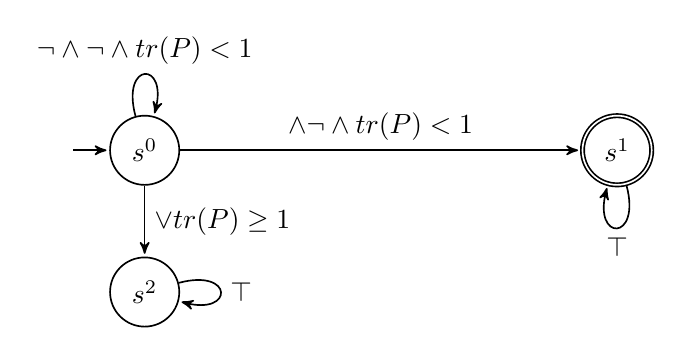
\begin{tikzpicture}[->,>=stealth',shorten >=1pt,auto,node distance=1.8cm, semithick,
initial text={}]
\tikzstyle{every state}=[text=black]

\node[initial,state]   (s0)                    {$s^0$};
\node[state,accepting] (s1) [right of=s0, node distance=6cm] {$s^1$};
\node[state]           (s2) [below of=s0] {$s^2$};

\path[->] (s0) edge [loop above] node {$\neg \goal \land \neg \obst \land tr(P) < 1$} (s0)
          (s0) edge node {$\goal \land \neg \obst \land tr(P) < 1$} (s1)
          (s1) edge [loop below] node {$\True$} (s1)
          (s0) edge node {$\obst \lor tr(P) \geq 1$} (s2)
          (s2) edge [loop right] node {$\True$} (s2);
\end{tikzpicture}
\caption{The FSA corresponding to Eq.~\eqref{eq:simple-spec}.}
\label{fig:simple-spec-fsa}
\end{figure}

\let\goal\undefined
\let\obst\undefined

%%%%%%%%%%%%%%%%%%%%%%%%%%%%%%%%%%%%%%%%%%%%%%%%%%%%%%%%%%%%%%%%%%%%%%%%
\subsection{Sampling-based methods in belief space}\label{sec:FIRM}
Motion planning problems in belief space $\CA{B}$ suffer from not only the curse of dimensionality but also the curse of history \cite{Pineau03a}. Further, planning in the joint belief and specification space (i.e., $\CA{B} \times \FSA$) makes this problem even harder. To ameliorate the curse of dimensionality and break the curse of history in POMDPs, we rely on recently developments in sampling-based methods in belief space. In particular, we use Feedback-based Information RoadMap (FIRM)~\cite{Agha14}, that uses local feedback controllers to break the curse of history associated with the POMDP. 

\begin{definition}[FIRM]
A Feedback-based Information RoadMap (FIRM) is a graph in belief space $\TS = (\TSX, \TSE, B^0)$, where $\TS$ represents a set of nodes in belief space $\TSX$ and the edge corresponds to a \sofie{[change to local feedback controller/mapping]} feedback local controller $\mu^{ij} \in \TSE$, which drives the system from belief node $B^i$ to $\epsilon$-neighbourhood of $B^j$ in finite time. The initial belief node is denoted by $B^0$. Note that each FIRM edge is a local controller, i.e., $\mu^{ij}:\mathbb{B}\rightarrow\mathbb{U}$.
\end{definition}

FIRM iteratively grows a graph $\TS$ in belief space, where each vertex/node corresponds to a Gaussian belief state $b = (\hat{x},P) \in \TSX$ with mean $\hat{x}$ and covariance $P$ \cite{Agha14}. For more details about sampling-based algorithms, and their connection to formal methods see~\cite{Lav06,KF-IJRR11,VaBe-IROS-2013}. %In Alg.~\ref{alg:compute-mdp}, edge controllers are generated using the method $localController()$.


% Prev Version --------
% In our approach, we use sampling-based techniques to generate paths throughout the state space. Sampling-based methods allow us to ameliorate the curse of dimensionality in traditional LTL-based methods (e.g., cell-decomposition TODO:\cite{}).
% To handle uncertainty in planning, in this work we rely on sampling-based techniques in belief space. Specifically, we propose a sampling-based algorithm to solve Pb.~\ref{pb:mpp} that overcomes the curse of dimensionality and history generally associated with POMDPs.

% In short, the sampling-based algorithm iteratively grows a graph $\TS$
% in the state space, where nodes are individual states, and edges 
% correspond to motion primitives that drive the system from state to state \cite{Ali14-IJRR}.

% %\cite{Lav06}.
% The extension procedure is biased towards exploration of
% uncovered regions of the state space.
% Similar to~\cite{Agha14}, we adapt sampling-based
% methods to produce finite abstractions (e.g., graphs) of the belief space.
% Alg.~\ref{alg:compute-mdp} incrementally constructs
% the transition belief graph FIRM $\TS = (\TSX, \BB{M}_\TS, B_0, \BB{E}_\TS)$,
% where $\TSX$ is the set of generated belief nodes,
% $ \BB{E}_\TS$ is the set of edges, and $\BB{M}_\TS$ is a set
% of controllers associated with edges.
% The belief nodes $b=(\hat{x}, P)\in\mathbb{V}$ are sampled from the reachable set of beliefs \cite{Agha14}.

% For more details about sampling-based algorithms, and how the graph can be generated see~\cite{Lav06,KF-IJRR11,VaBe-IROS-2013}.
% Transitions are enforced using local controllers which are stored
% in $\BB{M}_\TS$. i.e., we assign to the $(i,j)$-th edge
% a local controller denoted by $\mu^{ij} \in \BB{M}_\TS$. Under the assumptions of our model~\cite{Agha14}, the local controllers are guaranteed to stabilize the system to an $\epsilon$-neighborhood of belief nodes in finite time. Thus the transitions on the belief space is abstracted to transitions on the FIRM graph $\TS$. In Alg.~\ref{alg:compute-mdp}, edge controllers are generated using the method $localController()$.

% Prev Version --------

% center of a belief node is a belief state $b=(x, P^\infty)$,
% where the mean $x$ is obtained through random sampling of
% the system's state space, and $P^\infty$ is the stationary covariance.
% Sampling-based algorithms are built using a set of primitive
% functions that are assumed to be available:
% %The primitive functions we assume to be available are:
% \begin{itemize}
%   \item $sample(\CA{X})$ generates random states
% from a distribution over the state space $\CA{X}$,
%   \item $nearest(x^r, \TS) = \arg\min_{x^u}\{ \normeucl{x^r-x^u} \,|\, \exists P^u \wedge N_\delta(x^u, P^u) \in \TSX \}$
%   returns the mean $x^u$ of a belief node's center in $\TS$ such that $x^u$ is closest
%   to the state $x^r$ using the metric defined on $\CA{X}$,
%   \item $near(B_n, \TSX, \gamma)$ returns the closest $\gamma$
% belief nodes in $\TSX$ to $B_n$ with respect to the distance between their centers
% induced by $\norm{\cdot}_\CA{G}$, and
%   \item $steer(x^i, x^t)$ returns a state obtained by
% attempting to drive the system from $x^i$ towards $x^t$.
% \end{itemize}
% %For simplicity, in this paper we assume that the $steer()$
% %function is always able to produce a state that is closer
% %to $x_t$ that $x_i$ with respect to the metric defined on
% %$\CA{X}$.
% Using these primitive functions, an extension procedure
% $extend(\CA{X}, \TS)$ of the transition system $\TS$
% can be defined as:
% \begin{enumerate}
%   \item generate a new sample $x^r \asgn sample(\CA{X})$,
%   \item find nearest state $x^u \asgn nearest(x^r, \TS)$, and
%   \item drive the system towards the random sample
% $x^n \asgn steer(x^u, x^r)$.
% \end{enumerate}
%The design of the node controllers is presented Sec.~\ref{sec:caseStudy}. 

%However, when we plan to compute a policy to enforce the specification,
%we must compute the probability of invalidating the specification
%before stabilizing at a subsequent belief node.
%For this reason, we annotate the edges of the product automaton with
%``failure probabilities" (intersection) and transform it to an MDP.
%The intersection probabilities at the same time as the transition
%probabilities between the states of the MDP, i.e., pairs of belief nodes
%and DRA states.

%%%%%%%%%%%%%%%%%%%%%%%%%%%%%%%%%%%%%%%%
%A product MDP $\PA$
%between the TS $\TS$ and the DRA $\RA$ is
%maintained in an incremental fashion.
%The MDP captures motion and satisfaction at the same time, and 
%is used to compute the maximum probability satisfying policy $\mu^*$
%on the finite abstraction $\TS$.

%\begin{algorithm}
%\caption{$extend(\TS)$}
%\label{alg:extend}
%\DontPrintSemicolon
%\KwIn{$\TS$ -- belief transition system}
%\KwOut{$x_n$ -- random sample}
%\KwOut{$\Delta_n$ -- set of transitions}
%\BlankLine
%
%{\color{blue} TODO:}\;
%$done \asgn \False$\;
%\Repeat{$done$}{
%	
%}
%\Return $(x_n, \Delta_n)$
%\end{algorithm}

%\subsection{Local controllers}
%
%Similar to FIRM~\cite{Agha14}, we use local controllers
%to drive the system between the belief nodes of the
%transition system $\TS$, and to stabilize the belief about
%the system's state around the destination nodes.
%We assign to each node $B_i \in \TSX$ in the transition
%system a local controller $nc_i$, which drives the belief
%into $B_i$.
%We also associate with each transition
%$e = (B_u, B_v) \in \Delta_\TS$ an edge controller $ec_e$.
%The edge controller may simply be the node
%controller $nc_v$ associated with the destination node $B_v$.
%However, as suggested in~\cite{Agha14},
%two-stage local controllers are used instead.
%In the first stage, a
%pre-computed nominal trajectory is tracked until the system's state
%gets close to the destination belief node.
%Then, the controller switches to the node controller
%associated with the destination belief node.
%
%The design of the node controllers is presented Sec.~\ref{sec:caseStudy}. 
%For brevity, we omit the details of the tracking controller.
%{\color{blue} For more details about local controllers and examples using
%linear quadratic Gaussian techniques see~\cite{Agha14}.
%}
%It is shown in~\cite[Lemma 3]{Agha14} that these
%controllers can reach their destination belief nodes
%in finite (mean) time.

%\subsection{GDTL to LTL}
%\label{sec:gdtl2ltl}
%
%The predicates considered in GDTL
%are defined over the belief space $\CA{G}$ and
%describe sets in this space. However, because the
%uncertainty is separate from the temporal ordering
%of the satisfaction of the predicates, the sets
%determined by the predicates are independent
%of the position of a belief state $b^i$ in
%a belief word $\BF{b}$.
%As a consequence, we can convert a GDTL formula
%into an LTL formula.
%
%Denote $\CA{G}_f = \{ b\in \CA{G} \ |\ f(b) \leq 0\}$,
%where $f \in \CA{F}(\CA{G}, \BB{R})$.
%
%\begin{definition}[LTL Equivalent]
%\label{def:gdtl2ltl}
%Let $\phi$ be a GDTL formula and $F_\phi$ be the set
%of all predicates in $\phi$. Let $\AP$ be a finite set such
%that $\card{\AP} = \card{F_\phi}$ and a bijective
%map $\widetilde{\ }: F_\phi \to \AP$.
%Consider the LTL formula $\varphi$, where
%each predicate in $F_\phi$ is substituted by its associated
%atomic proposition in $\AP$ using the map
%$\widetilde{\ }$.
%The semantics of $\varphi$ are given with
%respect to infinite words in $\CA{G}^\omega$.
%Satisfaction of an atomic proposition
%$\BF{b} \models \widetilde{p}$ is interpreted as
%$b^0 \in \CA{G}_f$, where $p=(f \leq 0)\in F_\phi$.
%The Boolean and temporal operators retain
%their usual meaning.
%\end{definition}

\begin{figure}[h!]
	%\vspace*{-20pt}
	\centering
	%\subimport*{figs/}{graph.tex}	
 	%\documentclass{standalone}
\usepackage{tikz}
\usetikzlibrary{positioning}
\begin{document}
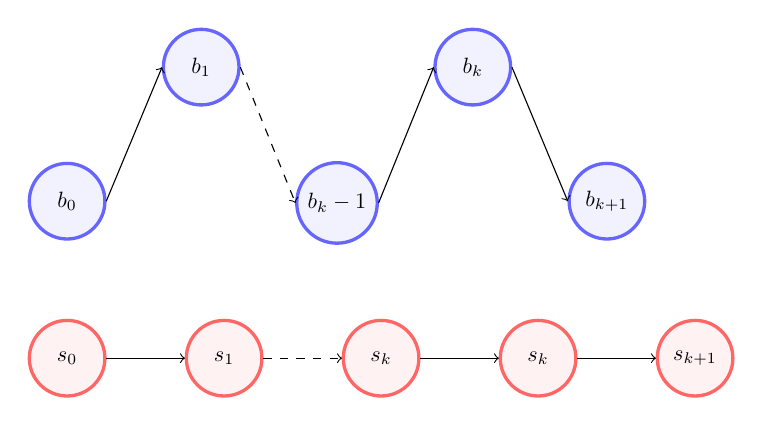
\begin{tikzpicture}[
beliefnode/.style={circle, draw=blue!60, fill=blue!5, very thick, minimum size=12mm},
rabinnode/.style={circle, draw=red!60, fill=red!5, very thick, minimum size=12mm}, every node/.style={scale=0.8}
]
% Belief path
%Nodes
\node[beliefnode]        (b0)                     {$b_0$};
\node[beliefnode]        (b1)       [above right=of b0] {$b_1$};
\node[beliefnode]        (b2)       [below right=of b1] {$b_k-1$};
\node[beliefnode]        (b3)       [above right=of b2] {$b_k$};
\node[beliefnode]        (b4)       [below right=of b3] {$b_{k+1}$};
%Lines
\draw[->] (b0.east) -- (b1.west);
\draw[dashed,->] (b1.east) -- (b2.west);
\draw[->] (b2.east) -- (b3.west);
\draw[->] (b3.east) -- (b4.west);
% Rabin Path
%Nodes
\node[rabinnode]        (s0)        [below=of b0]   {$s_0$};
\node[rabinnode]        (s1)        [right=of s0]   {$s_1$};
\node[rabinnode]        (s2)        [right=of s1]   {$s_k$};
\node[rabinnode]        (s3)        [right=of s2]   {$s_k$};
\node[rabinnode]        (s4)        [right=of s3]   {$s_{k+1}$};
%Lines
\draw[->] (s0.east) -- (s1.west);
\draw[dashed,->] (s1.east) -- (s2.west);
\draw[->] (s2.east) -- (s3.west);
\draw[->] (s3.east) -- (s4.west);


\end{tikzpicture}
\end{document}


	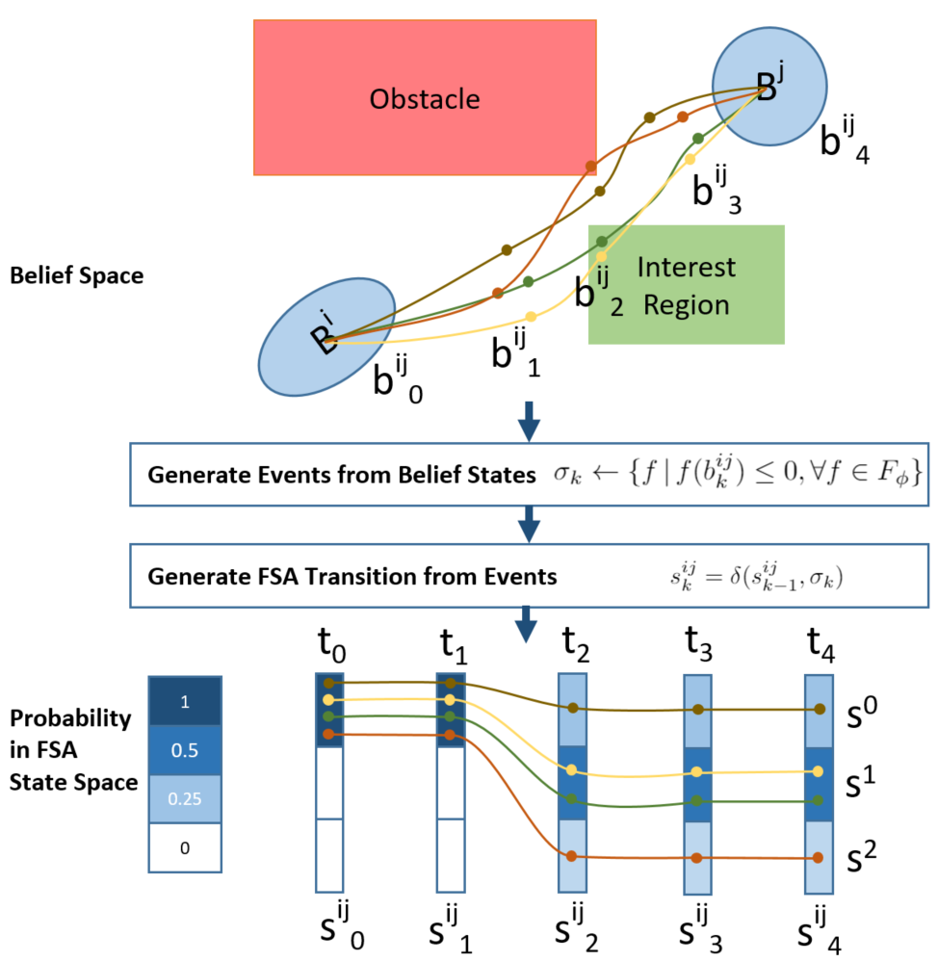
\includegraphics[width=\columnwidth]{figs/BeliefRabinTransitionV3.png}
	\caption{To compute transition probabilities in FSA state-space, we start with belief trajectories $b^{ij}_{0:4}$ (top) along a FIRM edge $\mu^{ij}$ obtained by sampling points in $B^i$ and simulating $\mu^{ij}$ controller until we reach $\epsilon-$neighborhood of $B^j$. For each $b^{ij}_k$ we find the event $\sigma_k$ fired by $b^{ij}_k$. The events $\sigma_k$ lead to the trajectory $S^{ij}_{0:4}$ in FSA state-space based on $s^{ij}_k = \delta(s^{ij}_{k-1},\sigma_k)$. Finally, we compute the transition probability in FSA state-space by computing the ratio of the number of particles that land in $s_k$ to the total number of particles simulated.}
	\label{fig:TransProb}
\end{figure}
%%%%%%%%%%%%%%%%%%%%%%%%%%%%%%%%%%%%%%%%%%%%%%%%%%%%%%%%%%%%%%%%%%
% \subsection{Rabin transition induced by belief transition}
% In this section, we discuss how a belief path will induce a specification path on the Rabin automaton.\\
% $s_0 \sim p(s_0)$,
% $s_k = T_{s_{k-1},b_{k}}^{s_k}(s_{k-1},b_k)$

% $T_{s_{k-1},b_{k}}^{s_k}$ passes $b_k$ through all predicates $2^{F_{\phi}}$ to get the input symbol (or event/letter) $\sigma_k$. We then use the transition function $\delta$ to get $s_k$ as shown below:

% $\sigma_k \asgn \{ f \,|\, f(b_k) \leq 0, \forall f \in F_\phi \}$,
% $s_k = \delta(s_{k-1},\sigma_k)$ \\


% % $\sigma_k \asgn \{ f \,|\, f(b^{ij}_k) \leq 0, \forall f \in F_\phi \}$,
% % $s^{ij}_k = \delta(s^{ij}_{k-1},\sigma_k)$

% Each sample transition $b_{0:n}^{ij}$ on the FIRM edge $\mu^{ij}$ induces a path on the Rabin Automaton $s_{0:n}^{ij}$

% $s_{0:k} = T_{s_0,b_{0:k}}^{s_{0:k}}(s_0,b_{0:k})$,
% $s_k = T_{s_0,b_{0:k}}^{s_k}(s_0,b_{0:k})$
% We overload $T$ for the all 3 transitions mentioned above.


%%%%%%%%%%%%%%%%%%%%%%%%%%%%%%%%%%%%%%%%%%%%%%%%%%%%%%%%%%%%%%%%%%
\subsection{Induced transition probabilities on FSA} \label{sec:TransProbSec}
In this section, we show how to estimate the FSA probability distribution induced by the underlying belief evolution on FIRM edges. 

The transitions in FSA are deterministic, i.e., FSA state $s_{i-1}$ with event $\sigma$ will always go to the same $s_{i}$. However, transitions in belief space are stochastic, i.e., belief $b_{i-1}$ with control input $u_{i}$ will not always go to the same $b_{i}$ due to stochasticity of observations.
%This is why we represent a belief as a probability distribution over the state space.
The probability distribution on FSA states is induced because of the stochasticity of the belief states.

Starting from initial belief $b_{0}$, and running the FIRM edge controller $\mu^{ij}$, belief evolves randomly due to the stochasticity of the observations. We denote the random belief sequence under $\mu^{ij}$ by $b_{0:n}^{ij}\sim p(b_{0:n}^{ij}|\mu^{ij},b_0)$, where $b_{0:n}^{ij}=(b_0^{ij},b_1^{ij},\cdots,b_n^{ij})$ (top graph in Fig. \ref{fig:TransProb}).

This belief distribution induces a distribution over FSA paths $s_{0:n}^{ij}\sim p(s_{0:n}^{ij}|\mu^{ij},s_0)$. 
In this work, we only work with the marginal distribution over the terminal state of the FSA path $p(s_{n}^{ij})\sim p(s_{0:n}^{ij}|\mu^{ij},s_0)$. We compute distribution $p(s_{n}^{ij})$ via first sampling belief trajectories under FIRM edge $\mu^{ij}$ and project them to the FSA transitions via predicates (see Fig. \ref{fig:TransProb}).

Figure \ref{fig:TransProb} shows a simple example illustrating how we compute the final FSA state distribution $p(s^{ij}_n|\mu^{ij},s_0)$.
We start from the belief $b_0$ at FIRM node $B^i$ and simulate the belief trajectory $b^{ij}_{0:n}$ by executing controller $\mu^{ij}$. We do this multiple times to create multiple belief paths. For each belief trajectory $b^{ij}_{0:n}$, we obtain the induced FSA trajectory $s^{ij}_{0:n}$ by first generating the event $\sigma_k \asgn \{ f \,|\, f(b^{ij}_k) \leq 0, \forall f \in F_\phi \}$ and then using the transition function $s^{ij}_{k} = \delta(s^{ij}_{k-1},\sigma_k)$. Finally, we approximate the $p(s^{ij}_n)$ by the ratio of the number of particles landed in a particular FSA state to the total number of particles simulated.

\sofie{[So actually, you use FIRM to find a good control sequence, which you then evaluate with a sampling based algorithm. Are you using any bounds on this? I added a reference \cite{Legay2010}. There has been done quite some work on this topic.]}
%Given a transition $e=(B_u, B_v)$ on the FIRM graph and its associated local controller $ec_e$,

% Alg.~\ref{alg:compute-prob} computes the above-mentioned transition distributions from an initial state $s_0$ on Rabin Automaton 

%to a some random DRA state, and a set
%of intersection distributions associated with each pair $(\CA{F}_i, \CA{B}_i)$
%of the acceptance set of $\RA$.


% In Alg.~\ref{alg:compute-prob}, the function $sampleBeliefSet(S)$
% returns a random sample from a uniform distribution over the
% belief set $S$.

% The distribution $\pi^{S_\RA}$ captures the probability that
% $s_v$ is the state of $\RA$ at the end of closed-loop
% trajectory generated by controller $ec_e$ to steer the system
% from belief node $B_u$ and DRA state $s_u$ to belief node $B_v$:
% $\pi^{S_\RA} = Pr[s_v \, |\, e, s_u, ec_e]$,
% where $s_v \in S_\RA$, $s_{u} \ras{\sigma_{0:T-1}} s_v$,
% $b^{0:T} = ec_e(b_u)$, $b_u \in B_u$, and
% $\sigma_k \asgn \{ f \,|\, f(b^k) \leq 0, \forall f \in F_\phi \}$.

% Each intersection distribution represents the probability that edge $e$
% intersects $\CA{F}_i$, $\CA{B}_i$ or neither, where
% $(\CA{F}_i, \CA{B}_i) \in \Omega_\RA$, and the controller $ec_e$
% was used to drive the system along the edge $e$ starting from
% the DRA state $s_u$:

% {\footnotesize
% \begin{align}
% \pi^{\Omega_\RA} = \left\{\left.
% \begin{cases}
% Pr[\BF{s}\cap \CA{F}_i \, |\, e, s_u, ec_e]\\
% Pr[\BF{s}\cap \CA{B}_i \, |\, e, s_u, ec_e]\\
% Pr[\BF{s}\cap (\CA{F}_i \cup \CA{B}_i) \, |\, e, s_u, ec_e]
% \end{cases}
% \,\right|\, \forall (\CA{F}_i, \CA{B}_i) \in \Omega_\RA \right\}
% \end{align}
% }%
% For convenience, we use the following notation
% $\pi^{\Omega_\RA}(e, X) = Pr[\BF{s}\cap X \, |\, e, s_u, ec_e]$,
% where $X \in \{\CA{F}_i, \CA{B}_i, \CA{F}_i \cup \CA{B}_i\}$.

%%%%%%%%%%%%%%%%%%%%%%%%%%%%%%%%%%%%%%%%%%%%%%%%%
\subsection{\DTL-FIRM Product MDP}\label{sec:DTL-FIRM}
The goal of this framework is to find the policy that maximizes the probability of satisfaction of the \DTL specification. For a partially observable system, the policy will generate the action based on the current belief in FIRM and current state in FSA. Formally, the policy $\mu=\pi(s,B)$, where $s$ the current FSA node and $B$ is the current FIRM node. The returned action is the local controller $\mu$.
%$\pi: \TSX \times S_\FSA \to \mathbb{E_\FSA}$ is a mapping from Cartesian product of the set of belief nodes in FIRM and FSA states to a FIRM edge, i.e., a feedback controller.
%We have $\pi^{FIRM}:B\rightarrow \mu$
To compute this policy in a computationally tractable manner, we define a construction procedure of the product MDP between the (belief) transition system (i.e., FIRM) $\TS$ and the FSA $\FSA$ generated from specifications.

\begin{definition}[\DTL-FIRM MDP]
\label{def:pa}
Given a FIRM graph $\TS = (\TSX, \TSE, B_0)$ and FSA $\FSA = (S_\FSA, s_0^\FSA, \Sigma, \delta_\FSA, Acc_\FSA)$ their product MDP is denoted by  $\PA = \TS \times \FSA$. Product MDP $\PA$
is a tuple $\PA = (Q_\PA, q_0^\PA, \TSE, \delta_\PA, Acc_\PA)$ where
$q_0^\PA = (B_0 , s_0^\FSA)$ is the initial state;
$Q_\PA \subseteq \TSX \times S_\FSA $ is a finite set of states, which are reachable from the initial state; % by run of positive probability (see below);
$\TSE$ is the set of actions available at each state;
$\delta_\PA : Q_\PA \times \TSE \times Q_\PA \ra [0, 1]$ is the transition probability
defined by $\delta_\PA((B^i, s^i), \mu^{ij}, (B^j, s^j))$. Goal set in the product space is defined as $Acc_\PA =  (\TSX \times Acc_\FSA) \cap Q_\PA$.
%= p^{S_\RA}(s_j ; e_{ij}, s_i, \CA{C}_\TS(e_{ij}))$, $e_{ij} = (B_i, B_j)$;
%and $\Omega_\PA$ is the set of tuples of good and bad transitions in the product automaton.

% Previous Def -------------------------------------------------------------------
% Given a DTS $\TS = (\TSX, B_0, \Delta_\TS, \CA{C}_\TS)$,
% a Rabin automaton $\RA = (S_\RA, s_0^\RA, \Sigma=\spow{\AP}, \delta, \Omega_\RA)$,
% and the transition and intersection probabilities $\pi^{S_\RA}$, $\pi^{\Omega_\RA}$,
% their product MDP, denoted by $\PA = \TS \times \RA$, is a tuple
% $\PA = (S_\PA, s_0^\PA, Act, \delta_\PA, \Omega_\PA)$ where %:
% $s_0^\PA = (B_0 , s_0^\RA)$ is the initial state;
% $S_\PA \subseteq \TSX \times S_\RA $ is a finite set of states
% which are reachable from the initial state by run of positive probability (see below);
% $Act = \TSX$ is the set of actions available at each state;
% $\delta_\PA : S_\PA \times Act \times S_\PA \ra [0, 1]$ is the transition probability
% defined by $\delta_\PA((B_i, s_i), B_j, (B_j, s_j)) = \pi^{S_\RA}(s_j ; e_{ij}, s_i, \CA{C}_\TS(e_{ij}))$, $e_{ij} = (B_i, B_j)$;
% and $\Omega_\PA$ is the set of tuples of good and bad transitions in the product automaton.

%\begin{itemize}
%    \item $s_0^\PA = (B_0 , s_0^\RA)$ is the initial state;
%    \item $S_\PA \subseteq \TSX \times S_\RA $ is a finite set of states
%    which are reachable from the initial state by run of positive probability (see below);
%    \item $Act = \TSX$ is the set of actions available at each state;
%    \item $\delta_\PA : S_\PA \times Act \times S_\PA \ra [0, 1]$ is the transition probability
%    defined by $\delta_\PA((B_i, s_i), B_j, (B_j, s_j)) = \pi^{S_\RA}(s_j ; e_{ij}, s_i, \CA{C}_\TS(e_{ij}))$, $e_{ij} = (B_i, B_j)$;
%    \item $\Omega_\PA$ is the set of tuples of good and bad transitions in the product automaton.
%\end{itemize}
\end{definition}

%    : for every $(x^*, s^*) \in S_\PA$ there exists a sequence of $\BF{x} = x_0 x_1 \ldots x_n x^*$, with $x_k \ra_\TS x_{k+1}$ for all $0 \leq k < n$ and $x_n \ra_\TS x^*$, and a sequence $\BF{s} = s_0 s_1 \ldots s_n s^*$ such that $s_0 = s_0^\RA$, $s_k \ras{h(x_k)}_\RA s_{k+1}$ for all $0 \leq k < n$ and $s_n \ras{h(x_n)}_\RA s^*$;

% Denote the set of edges of positive probability by
% $\TSEE_\PA = \left\{ \big((B^i, s^i), (B^j, s^j) \big) \,|\, \delta_\PA((B^i, s^i), \mu^{ij}, (B^j, s^j)) > 0 \right\}$.

%A transition in $\PA$ is also denoted by $q_i \ra_\PA q_j$ if $(q_i, q_j) \in \Delta_\PA$. A trajectory (or run) of {\em positive probability} of $\PA$ is an infinite sequence $\BF{q} = q_0 q_1 \ldots$, where $q_0 = q^\PA_0$ and $q_k \ra_\PA q_{k+1}$ for all $k \geq 0$.

The acceptance condition for a trajectory of product graph $\PA$ is encoded in
$Acc_\PA$, and is induced by the acceptance condition $Acc_\FSA$ of
FSA $\FSA$.
% Formally, $\Omega_\PA$ is a pair $(Acc_\PA, Bad_\PA)$,
% where 
% $Acc_\PA = \{ e \in \Delta_\PA \,|\, p(Acc_\FSA \mid e) > 0\}$, and
% $Bad_\PA = \{ e \in \Delta_\PA \,|\, p(Trap_\FSA \mid e) > 0\}$.
% {\color{red}what is $Acc_\FSA$? has been defined already?}
A trajectory of $\PA = \TS \times \FSA$ is said to be accepting
if and only if the trajectory ends in a state from $Acc_\PA$. The acceptance condition for $\PA$ is defined by its transitions and not in the usual way in terms of its states, due to the stochastic nature of transitions between belief nodes in $\TS$.
\sofie{[The last statement does not make sense to me, the acceptance condition is defined as $Acc_\FSA$ which is a subset of the states $Q_\PA $ of $\PA$]}
%It follows by construction that a trajectory $\BF{q} = (B_0, s_0) (B_1, s_1) \ldots$ of $\PA$ is accepting if and only if the trajectory $\BF{s}^0_{0:T_0-1} \BF{s}^1_{0:T_1-1} \ldots$ is accepting in $\FSA$, where $\BF{s}^i_{0:T_i}$ is the random trajectory of $\FSA$ obtained by traversing the transition $e = (B_i, B_{i+1})$ using the controller $\mu^{ij}$ and $s^i_{0} = s_i$ for all $i \geq 0$. Note that $\BF{s}^i_{T_i} = \BF{s}^{i+1}_0$. As a result, a trajectory of $\TS$ obtained from an accepting trajectory of $\PA$ satisfies the given specification encoded by $\FSA$ with positive probability. We denote the projection of a trajectory $\BF{q} = (B_0, s_0) (B_1, s_1) \ldots$ onto $\TS$ by $\proj{\BF{q}}{\TS} = B_0 B_1 \ldots$.

\begin{remark}
Note that the product MDP in Def.~\ref{def:pa} can be created incrementally as both FIRM graph $\TS$ and the FSA $\FSA$ can be constructed incrementally \cite{Agha14,VaBe-IROS-2013}.
\end{remark}

% \begin{remark}
% Note that the product MDP in Def.~\ref{def:pa} is defined to be amenable to
% incremental operations with respect to the growth of the $\TS$, i.e., updating and
% checking for a solution of positive probability.
% This property is achieved by requiring the states of $\PA$ to be reachable
% by transitions in $\Delta_\PA$.
% The incremental update can be performed using a recursive procedure
% similar to the one described in~\cite{VaBe-IROS-2013}.
% \end{remark}
% \begin{remark}
% The acceptance condition for $\PA$ is defined by its transitions and not in the usual way in terms
% of its states, % the usual way.
% %The choice is
% due to the stochastic nature of transitions between belief
% nodes in $\TS$. %We only record the initial and end FSA states of the FSA trajectories induced by the sample paths obtained using the local controllers.
% \end{remark}

%Our construction is conservative, but avoids the need to store a (possibly large)
%number of intermediate states in $\PA$ for spurious sample paths % which deviate
%deviating
%from the nominal one.
%Thus, the burden of the search is shifted from the verification component
%of the solution, to the sampling-based search procedure.
%A heuristic argument for our choice is that most of the time sample paths
%swill generate the same DRA trajectory as the nominal path.



%For brevity, we omit its description and refer the reader to~\cite{VaBe-IROS-2013}.

% Satisfying policy is defined as policy that visits the good states initientely many time and bad state finitely many times. 
% In this section, we .... to compute a satisfying policy.

% The existence of a policy that can satisfy the specifications with positive probability can be checked efficiently
% on the product MDP $\PA$ by maintaining end components EC\footnote{An
% EC of an MDP is a sub-MDP  such that there exists a policy such that each
% node in the EC can be reached from each other node in the EC with positive
% probability.}
% for induced subgraphs of $\PA$ determined by the pairs in the acceptance
% condition $\Omega_\PA$.
% %An SCC is a subgraph such that each node in the SCC can be reached from each other node in the SCC.
% For each pair $\CA{F}^\PA_i, \CA{B}^\PA_i$, let $c_i$ denote the
% ECs associated with the graphs $G^\PA_i = (S_\PA,\Delta_\PA \setminus \Gamma_i)$, where
% $\Gamma_i =  \{ (p, p') \in \Delta_\PA \,|\, \pi^{\Omega_\RA}(e, \CA{F}_i) = 0 \wedge \pi^{\Omega_\RA}(e, \CA{B}_i) > 0, e=\proj{(p, p')}{\TS} \}$.
% %Let $dag_i$ be the directed acyclic graphs (DAGs) associated with $scc_i$.
% Given $c_i$, checking for a satisfying trajectory in procedure $existsSatPolicy(\PA)$
% becomes trivial.
% We test if there exists an EC %reachable in $dag_i$ from the SCC containing $s^\PA_0$
% that contains a transition $(p, p')$ such that
% $\pi^{\Omega_\RA}(e, \CA{F}_i) > 0$, where $e=\proj{(p, p')}{\TS}$.
% Note that we do not need to maintain $\Omega_\PA$ explicitly, we only
% need to maintain the  $c_i$.
% Efficient incremental algorithms to maintain these ECs were proposed
% in~\cite{Haeupler2012}. %,Bender2015

\begin{algorithm}[!h]
\caption{SynthesizeRoverPolicy$(B_0,\phi,\varepsilon)$ }
\label{alg:compute-mdp}
\DontPrintSemicolon
\KwIn{Initial belief node $B_0$, \DTL specification $\phi$, and lower bound $\varepsilon$ on the policy success probability}
%\KwIn{\color{blue} $(f, h)$ -- model of the robot (motion and sensing)}
%\KwIn{$\phi$ -- GDTL specification}
%\KwIn{$\varepsilon$ -- lower bound probability of satisfying policy}
\KwOut{Belief graph $\TS$, product MDP $\PA$, and satisfying policy $\pi^*$}
%\KwOut{$\PA$ -- product MDP}
%\KwOut{$\mu^* : S_\PA \to S_\PA$ -- satisfying feedback policy on $\PA$ w/ probability at least $\varepsilon$}
\BlankLine
Convert \DTL formula $\phi$ to LTL formula $\varphi$ over the set of atomic propositions $\AP=F_\phi$ (using \cite{JonesDTL2013})\;
%%%%
Compute FSA $\FSA = (S_\FSA, s_0, \Sigma, \delta_\FSA, Acc_\FSA)$ from $\varphi$ (using \cite{duret14})\;
%%%%
Initialize belief graph $\TS = (\TSX = \{B_0\}, \TSE = \emptyset, B_0)$\;
Construct product MDP $\PA = \TS \times \FSA = (S_\PA = \TSX \times S_\FSA, (B_0, s_0),
\TSE,\delta_\PA = \emptyset, Acc_\PA)$\;

\For{$iteration = 1$ \KwTo $N$}{
    Sample a belief node $B_n$ (using \cite{Agha14})\;
    Connect $B_n$ to FIRM graph via constructing new edges $\TSEE_n$ (using \cite{Agha14})\;
    $\TSX \asgn \TSX \cup \{B_n\}$, $\TSE \asgn \TSE \cup \TSEE_n$\;
    $S_\PA \asgn S_\PA \cup (\{ B_n \} \times S_\FSA)$\;
    \ForEach{$\mu^{i j} \in \TSEE_n$}{
        \ForEach{$s^i \in S_\FSA$ s.t. $(B^i, s^i) \in S_\PA$}{
            $p(b_{n}^{ij}), p(s_{n}^{ij}) \asgn transProb((b^i,s^i), \mu^{ij},\FSA)$ (using Sec. \ref{sec:TransProbSec})\;
            %%%
            $\delta_\PA \asgn \delta_\PA \cup \{ p(b_{n}^{i j}) \times p(s_{n}^{i j}) \}$\;
        }
    }
    % $\Delta^n_\PA = \{ (p, p') \in \Delta_\PA \,|\, \proj{(p, p')}{\TS} \in \Delta_n \}$\;
    % \ForEach(\tcp*[h]{update ECs}){$(\CA{F}_i, \CA{B}_i) \in \Omega_\FSA$}{
    %     $\begin{aligned}\Gamma_i &= \{ (p, p') \in \Delta^n_\PA \,|\, \pi^{\Omega_\FSA}(e, \CA{F}_i) = 0 \\
    %     &\qquad {} \wedge \pi^{\Omega_\FSA}(e, \CA{B}_i) > 0, e=\proj{(p, p')}{\TS} \} \end{aligned}$\;
    %     $c_i.update(\Delta^n_\PA \setminus \Gamma_i)$\;
    % }

%    {\color{blue} update SCCs' reach and stay probabilities}\;

    %\If{$Acc_\PA \neq \emptyset$}{
    $Acc_\PA \asgn updateGoalState( \TSX, \FSA )$ using Def. \ref{def:pa}\;
    \If{$Acc_\PA \neq \emptyset$}{
        Solve DP and compute policy $\pi^*$ using Eq.~\eqref{eq:product-DP}\;
        Compute probability of satisfaction $p$\;
        \lIf{$p \geq \varepsilon$}{
            \Return $(\PA, \pi^*)$
        }
    }
}
\Return $(\PA, \emptyset)$
\end{algorithm}

\begin{algorithm}
\caption{ExecuteCampaign($B_0, \phi, \varepsilon$)}
\label{alg:execute}
\DontPrintSemicolon
\KwIn{Initial belief node $B_0$, \DTL specification $\phi$, and lower bound $\varepsilon$ on the policy success probability}
$m$ = $\emptyset$ \\
$\bar{m} \asgn$ GetInitialExplorationDirection() \\
\For{ever}{
    $m \asgn$  ExploreMapUsingCopter($m,\bar{m}$) \\
    $m^l \asgn$ UpdateLabels($m$) \\
    $\phi \asgn$ UpdateRegionsInSpecification($m^l$) \\
    $(\PA, \pi) \asgn$ $SynthesizeRoverPolicy(B_0,\phi,\varepsilon)$ \label{plan}\\
    \If{$\pi \neq \emptyset$}{
        $(success, health) \asgn$ ExecuteRoverPolicy$ (\PA, \pi^*,\phi)\ $\\
        \If{$success = true$}{
            \Return{success};
        }
        \Else{
            $\phi \asgn$ UpdateSpecification($health$)\\
            \textbf{Goto} line~\ref{plan}\\
        }
    }
    \Else{
        $\bar{m} \asgn$ GetExplorationDirection($\PA, \pi, m$)
    }
}
\BlankLine
\end{algorithm}

% \begin{algorithm}
% \caption{$computeProb(e=(B_u, B_v), s_u, ec_e, \RA)$ TODO: Remove}
% \label{alg:compute-prob}
% \DontPrintSemicolon
% \SetKwInOut{KwParam}{Parameter}
% \KwIn{transition between belief nodes $e=(B_u, B_v)$, starting DRA state $s_u$, controller enforcing $e$ $ec_e$, and deterministic Rabin automaton $\RA$}
% %\KwIn{$s_u$ -- starting DRA state}
% %\KwIn{$ec_e$ -- controller enforcing $e$}
% %\KwIn{$\RA$ -- deterministic Rabin automaton}
% \KwOut{transition distribution $\pi^{S_\RA}$, and intersection distribution $\pi^{\Omega_\RA}$ }
% %\KwOut{$\pi^{\Omega_\RA}$ -- reach/avoid distribution}
% \KwParam{$NP$ -- number of particles}
% \BlankLine

% $t \asgn \BF{0}_{\card{S_\RA}, 1}$\;
% $ra_i \asgn \BF{0}_{3, 1}$, $\forall (\CA{F}_i, \CA{B}_i) \in \Omega_\RA$\;
% \For{$p=1:NP$}{
%     $b_u \asgn sampleBeliefSet(B_u)$\;
%     $b^{0:T} \asgn ec_e(b_u)$\;
%     \For{$k = 0$ \KwTo $T-1$}{
%         $\sigma_k \asgn \{ f \,|\, f(b^k) \leq 0, \forall f \in F_\phi \}$\;
%     }
%     $\BF{s} = s_{0:T} \asgn (s_u \ras{\sigma_{0:T-1}} s_T)$\;
%     $t[s_T] \asgn t[s_T] + 1$\;
%     \For{$(\CA{F}_i, \CA{B}_i) \in\card{\Omega_\RA}$}{
%         \lIf{$\CA{F}_i \cap \BF{s} \neq \emptyset$}{
%             $ra_i[1] \asgn ra_i[1] + 1$
%         }
%         \lIf{$\CA{B}_i \cap \BF{s} \neq \emptyset$}{
%             $ra_i[2] \asgn ra_i[2] + 1$
%         }
%         \lIf{$(\CA{F}_i \cup \CA{B}_i)\cap \BF{s} = \emptyset$}{
%             $ra_i[3] \asgn ra_i[3] + 1$
%         }
%     }
% }
% \Return $\left( \pi^{S_\RA} = \frac{t}{NP}, \pi^{\Omega_\RA} = \left\{ \frac{ra_i}{NP} \,|\, 1\leq i\leq \card{\Omega_\RA} \right\} \right)$
% \end{algorithm}


%%%%%%%%%%%%%%%%%%%%%%%%%%%%%%%%%%%%%%%%%%%%%%%%%%%%%%%%%%%%%%%%%%%%%%%%%
\subsection{Finding the Maximum Probability policy}
The existence of satisfying policies results immediately from the construction.
\sofie{[This isn't obvious to me]}
We only need to check if the product MDP $\PA$ has any accepting transitions $Acc_\PA$.

Given a \DTL-FIRM MDP, we can compute the optimal switching policy to maximize the probability that a given formula $\phi$ is satisfied.  
%%
%This is done by solving the following optimization problem
%
%\begin{equation}
%\label{probMax}
%	\underset{m \in \mathcal{F}(S_{\mathcal{P}},Act)}{\arg \max} \bigwedge_{i\in \Omega_{\mathcal{R}}}\bigwedge_{j=1}^\infty Pr_{m}( \bigvee_{k=1}^{\infty} s_{j+k} \cap \mathcal{F}_i \wedge s_{j+k} \in S_{\mathcal{P}} \setminus B_i) 
%\end{equation}
%
In other words, we find a policy that maximizes the probability of visiting the $Acc_\PA$ states.
% To find this policy, we first decompose $\mathcal{P}$ into a set of end components and find the accepting components. Since any sample path that satisfies $\phi$ must end in an accepting component, maximizing the probability of satisfying $\phi$ is equivalent to maximizing the probability of reaching such a component.
The optimal policy is thus given by the relationship
%{\footnotesize
% \begin{equation}
% \label{eq:dp}
% \resizebox{0.90\columnwidth}{!}{
% $\begin{array}{lcl}
% J^{\infty}(s) &=& \left \{ \begin{array}{ll}
% 1, &  s \in c_i \\ 
% \underset{a \in Act(s)}{\max} \sum_{s'} \delta(s,a,s')J^{\infty}(s') & \text{else} 
% \end{array} \right .  \\
% m(s) &=& \underset{a \in Act(s)}{\arg \max} \sum_{s'} \delta(s,a,s')J^{\infty}(s') \\
% \end{array}$}
% \end{equation}
\begin{align}
J(s) &= \begin{cases}
1, &  s \in Acc_\PA \\ 
\underset{\mu \in \mathbb{M}(s)}{\max} \sum_{s'} \delta(s,\mu,s')J(s') & \text{otherwise} 
\end{cases}  \label{eq:product-DP}\\
\pi(s) &= \underset{\mu \in \mathbb{M}(s)}{\arg \max} \sum_{s'} \delta(s,\mu,s')J(s')
\end{align}

%}
\sofie{[This is only holds if $J$ is either initialized with zero, and then iterated. Additionally, you are of course not computing the maximal policy. At least, there is no prove that you are. Since you are working with probability transitions which are estimates of the actual probability distribution. This is totally fine, just clarify.]}
The value function $J(\cdot)$ can be computed by solving the Eq.~\ref{eq:product-DP} via a variety of methods, including approximate value iteration and linear programming~\cite{Bertsekas2012}.
\sofie{See previous statement, I disagree with the notion that this can be solved with LP. The operator (for LP) defined in (18) is not contractive!  You can only show that it will converge if you start at zero, since in that case it is strictly increasing. Probably there are some conditions in one of the papers of Ilya Tkachev that states on which conditions contractivity can be assumed. Anyways, as a counter example. Take a trivial MDP, with a unreachable accepting state and a circle connection of deterministic transitions. Put one value of this cycle to 1, then at each iteration the state with value 1 will move one position. This issue can probably be fixed by requiring that J is the smallest positive solution of the bellman equation.}
%[Cite Bertsekas]


%\subsection{Querying the FIRM}

%%%%%%%%%%%%%%%%%%%%%%%%%%%%%%%%%%%%%%%%%%%%%%%%%%%
\subsection{Algorithm}%Checking 

%%%%%%%%%%%%%%%%%%%%%%%%%%%%%%%%%%%%%%%%%%%%%%%%%%%%%%%%%%%%%%%%%%%%%%%%%
\subsubsection{Execution, remapping, and replanning} \label{replanning}

\cristi{Need to add description of the execution copter and rover,
remapping triggering and information passed between rover and copter, and replanning
for the rover}

%%%%%%%%%%%%%%%%%%%%%%%%%%%%%%%%%%%%%%%%%%%%%%%%%%%%%%%%%%%%%%%%%%%%%%%%%
\subsubsection{Complexity}\label{complexity}
% The overall complexity of maintaining the ECs used for checking
% for satisfying runs in $\PA$ is $O(\card{\Omega_\RA} \card{S_\PA}^{\frac{3}{2}})$~\cite{Haeupler2012} and is better by a polynomial factor
% $\card{S_\PA}^{\frac{1}{2}}$ than computing the ECs at each
% step using a linear algorithm.
Checking for the existence of a satisfying run of positive probability
can be done in $O(1)$ time.
The dynamic programming algorithm is polynomial in
$\card{S_\PA}$~\cite{papadimitriou1987}.

%{\color{blue} [To be written by Cristi]
%
%For all TS, DRA and MDP, we use $\card{\cdot}$ to denote size,
%which is the cardinality of the corresponding set of states.
%
%\begin{itemize}
%  \item the overall complexity of maintaining the SCCs is $O(\card{\Omega_\RA} n^{\frac{3}{2}})$, where $\card{\TS} \leq n = \card{\PA} \leq \card{\TS} \cdot \card{\RA}$, if:
%  \begin{itemize}
%    \item $\TS$ is a sparse graph; and
%    \item the incremental SCC algorithm used to update the SCCs has overall complexity $O(n^{\frac{3}{2}})$.
%  \end{itemize}
%  \item the first part of the test can be checked in $O(1)$ if one maintains $F_\PA$, which resembles the case of a product with a \buchi
%  \item the complexity of checking for the existence of satisfying path is $O(\card{\Omega_\RA})$
%\end{itemize}
%
%}

%\subsection{Conclusion of Running Example}
	

	%%%%%%%%%%%%%%%%%%%%%%%%%%%%%%%%%%%%%%%%%%%%%%%%%%%%%%%%%%%%%%%%%%%%%%%%
	\section{Results} \label{sec:simulation}
	
% 	\begin{figure}[ht!]
% 		\centering
% 		\subfigure{
% 		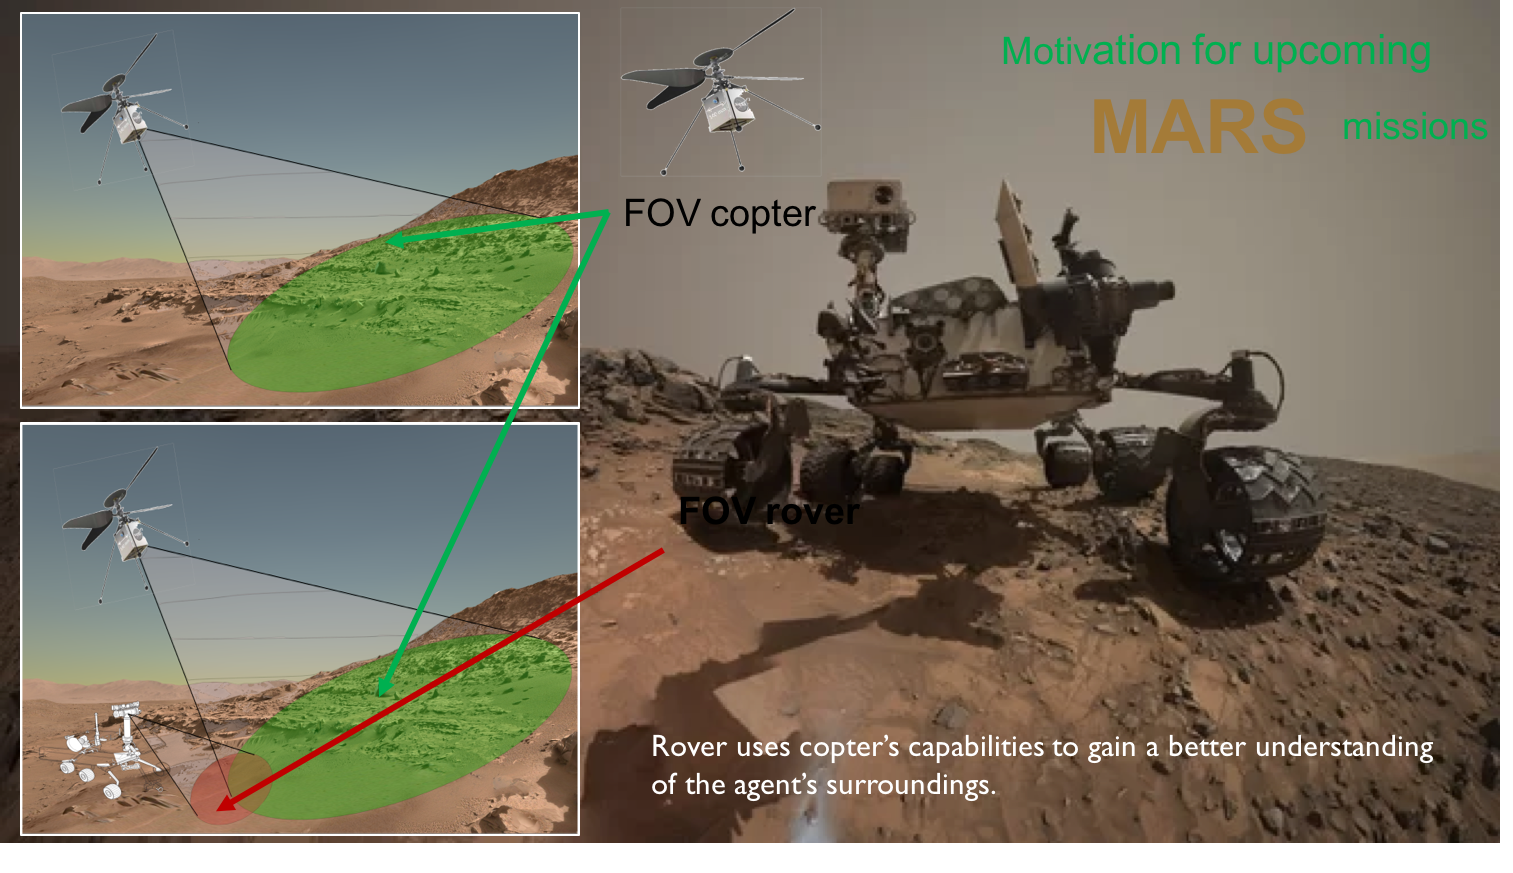
\includegraphics[width=.7\columnwidth,trim=5.cm 1.cm 4.cm 1.cm,clip]{FOV.png}\vspace{-16pt}
% 		\label{fig:bad_error_consistency}}
% 		\caption{Mapping error (red) and algorithmically computed std deviation (blue shades for $ 2\sigma $ (light) and $ \sigma $ (dark) confidence bounds) over a set of voxels, with highlighted severe inconsistencies (black rectangles). Top row corresponds to the proposed method and bottom row corresponds to the log-odds method.}
% 	\end{figure}		
	
	
	%%%%%%%%%%%%%%%%%%%%%%%%%%%%%%%%%%%%%%%%%%%%%%%%%%%%%%%%%%%%%%%%%%%
	\section{Conclusion} \label{sec:conclusion}
	This paper proposes ...
	
	%%%%%%%%%%%%%%%%%%%%%%%%%%%%%%%%%%%%%%%%%%%%%%%%%%%%%%%%%%%%%%%%%%%
 
	    
	
	%Similar to research toward joint design of localization and planning frameworks (e.g., \cite{Ali14-IJRR}), this work paves the way for future studies on tighter integration of planning and mapping methods. In such joint design, the map uncertainty can play a crucial role in planning and task-oriented acquisition of perceptual information.
	
	%%%%%%%%%%%%%%%%%%%%%%%%%%%%%%%%%%%%%%%%%%%%%%%%%%%%%%%%%%%%%%%%%%%%%%%%%%%%%%%%
	
	%\bibliographystyle{ieeeTran} %\bibliographystyle{apalike}
	
	\bibliographystyle{plain}
	\bibliography{AliAgha,references}
	%\bibliography{references.bib}
	
	%%%%%%%%%%%%%%%%%%%%%%%%%%%%%%%%%%%%%%%%%%%%%%%%%%%%%%%%%%%%%%%%%%%%%%%%%%%%%%%%
% 	\begin{appendices}
		
% 		%%%%%%%%%%%%%%%%%%%%%%%%%%%%%%%%%%%%%%%%%%%%%%%%%%%%%%%%%%%%%%%%%%%%%%%%
% 		\section{Proof of Lemma \ref{lem:cause-meas}} \label{app:proofLemma}
% 		\begin{align}
% 		\nonumber
% 		&p(m^i|c_k,z_{0:k},xv_{0:k})
% 		\\
% 		\nonumber
% 		&=
% 		\frac{p(z_k|m^i,c_{k},z_{0:k-1},xv_{0:k})p(m^i|c_{k},z_{0:k-1},xv_{0:k})}
% 		{p(z_k|c_{k},z_{0:k-1},xv_{0:k})}
% 		\\
% 		\nonumber
% 		&=
% 		\frac{p(z_k|c_{k},z_{0:k-1},xv_{0:k})p(m^i|c_{k},z_{0:k-1},xv_{0:k})}
% 		{p(z_k|c_{k},z_{0:k-1},xv_{0:k})}
% 		\\
% 		\nonumber &=
% 		p(m^i|c_{k},z_{0:k-1},xv_{0:k})
% 		\end{align}
		
% 		%%%%%%%%%%%%%%%%%%%%%%%%%%%%%%%%%%%%%%%%%%%%%%%%%%%%%%%%%%%%%%%%%%%%%%%%
% 		%\section{title}
% 		%\begin{align}
% 		%\nonumber
% 		%&p(c_{k} | z_{0:k-1},xv_{0:k}) = 
% 		%\Pr(B^{c_{k}},R^{c_{k}}| z_{0:k-1},xv_{0:k}) \\
% 		%\nonumber
% 		%&= \Pr(B^{c_{k}} |  z_{0:k-1},xv_{0:k})\Pr(R^{c_{k}}|B^{c_{k}}, z_{0:k-1},xv_{0:k})
% 		%\end{align}
		
		
% 	\end{appendices}

\end{document}

